% Soubory musí být v kódování, které je nastaveno v příkazu \usepackage[...]{inputenc}

\documentclass[%
%  draft,    				  % Testovací překlad
  12pt,       				% Velikost základního písma je 12 bodů
  a4paper,    				% Formát papíru je A4
%  oneside,      			% Jednostranný tisk (výchozí)
%% Z následujicich voleb lze použít maximálně jednu:
%	dvipdfm  						% výstup bude zpracován programem 'dvipdfm' do PDF
%	dvips	  						% výstup bude zpracován programem 'dvips' do PS
%	pdftex							% překlad bude proveden programem 'pdftex' do PDF (výchozí)
%% Z následujících voleb lze použít jen jednu:
%english,            % originální jazyk je angličtina
czech              % originální jazyk je čeština (výchozí)
%slovak,             % originální jazyk je slovenčina
]{report}				    	% Dokument třídy 'zpráva'

\usepackage[utf8]		%	Kódování zdrojových souborů je Windows-1250
	{inputenc}					% Balíček pro nastavení kódování zdrojových souborů

\usepackage{graphicx} % Balíček 'graphicx' pro vkládání obrázků
											% Nutné pro vložení log školy a fakulty

\usepackage{xcolor,colortbl} % Hyna
\usepackage{subcaption} % Hyna

\usepackage[
	nohyperlinks				% Nebudou tvořeny hypertextové odkazy do seznamu zkratek
]{acronym}						% Balíček 'acronym' pro sazby zkratek a symbolů
											% Nutné pro použití prostředí 'seznamzkratek' balíčku 'thesis'

\usepackage[
	unicode,						% Záložky a informace budou v kódování unicode
	breaklinks=true,		% Hypertextové odkazy mohou obsahovat zalomení řádku
	hypertexnames=false % Názvy hypertextových odkazů budou tvořeny
											% nezávisle na názvech TeXu
]{hyperref}						% Balíček 'hyperref' pro sazbu hypertextových odkazů
											% Nutné pro použití příkazu 'nastavenipdf' balíčku 'thesis'

\usepackage{pdfpages} % Balíček umožňující vkládat stránky z PDF souborů
                      % Nutné při vkládání titulních listů a zadání přímo
                      % ve formátu PDF z informačního systému

\usepackage{enumitem} % Balíček pro nastavení mezerování v odrážkách
  \setlist{topsep=0pt,partopsep=0pt,noitemsep}

\usepackage{cmap} 		% Balíček cmap zajišťuje, že PDF vytvořené `pdflatexem' je
											% plně "prohledávatelné" a "kopírovatelné"

\usepackage{upgreek}	% Balíček pro sazbu stojatých řeckých písmem
											% např. stojaté pí: \uppi
											% např. stojaté mí: \upmu (použitelné třeba v mikrometrech)
											% pozor, grafická nekompatibilita s fonty typu Computer Modern!

%% Nastavení českého jazyka při sazbě v češtině.
% Pro sazbu češtiny je možné použít mezinárodní balíček 'babel', jenž
% použití doporučujeme pro nové instalace (MikTeX2.8,TeXLive2009), nebo
% národní balíček 'czech', který doporučujeme ve starších instalacích.
% Balíček 'babel' bude správně fungovat pouze ve spojení s programy
% 'latex', 'pdflatex', zatímco balíček 'czech' bude fungovat ve spojení
% s programy 'cslatex', 'pdfcslatex'.
% Varianta A:
\usepackage{babel}             % Balíček pro sazbu různojazyčných dokumentů; kompilovat (pdf)latexem!
  										% převezme si z parametrů třídy správný jazyk
\usepackage{lmodern}	% vektorové fonty Latin Modern, nástupce půvoních Knuthových Computern Modern fontů
\usepackage{textcomp} % Dodatečné symboly
\usepackage[T1]{fontenc}  % Kódování fontu - mj. kvůli správným vzorům pro dělení slov
% Varianta B:
%\usepackage{czech}   % Alternativní balíček pro sazbu v českém jazyce, kompilovat (pdf)cslatexem!

\usepackage[%
%% Z následujících voleb lze použít pouze jednu
% left,               % Rovnice a popisky plovoucich objektů budou %zarovnány vlevo
  center,             % Rovnice a popisky plovoucich objektů budou zarovnány na střed (vychozi)
%% Z následujících voleb lze použít pouze jednu
%semestral						%	sazba zprávy semestrálního projektu
%bachelor						%	sazba bakalářské práce
diploma						 % sazba diplomové práce
%treatise            % sazba pojednání o dizertační práci
%phd                 % sazba dizertační práce
]{thesis}             % Balíček pro sazbu studentských prací
                      % Musí být vložen až jako poslední, aby
                      % ostatní balíčky nepřepisovaly jeho příkazy

%%%%%%%%%%%%%%%%%%%%%%%%%%%%%%%%%%%%%%%%%%%%%%%%%%%%%%%%%%%%%%%%%
%%%%%%      Definice informací o dokumentu             %%%%%%%%%%
%%%%%%%%%%%%%%%%%%%%%%%%%%%%%%%%%%%%%%%%%%%%%%%%%%%%%%%%%%%%%%%%%

%% Název práce:
%  První parametr je název v originálním jazyce,
%  druhý je překlad v angličtině nebo češtině (pokud je originální jazyk angličtina)
\nazev{Sekvenční osazování povrchově montovaných součástek}{Sequential Placement of Surface Mounted Devides}

%% Jméno a příjmení autora ve tvaru
%  [tituly před jménem]{Křestní}{Příjmení}[tituly za jménem]
\autor[Bc.]{Hynek}{Štětina}

%% Jméno a příjmení vedoucího včetně titulů
%  [tituly před jménem]{Křestní}{Příjmení}[tituly za jménem]
\vedouci[Ing.]{Jiří}{Starý}[Ph.D.]

%% Označení oboru studia
% První parametr je obor v originálním jazyce,
% druhý parametr je překlad v angličtině nebo češtině
\oborstudia{Mikroelektronika}{Microelectronics}

%% Označení ústavu
% První parametr je název ústavu v originálním jazyce,
% druhý parametr je překlad v angličtině nebo češtině
\ustav{Ústav mikroelektroniky}{Department of Microelectronics} 

%% Rok obhajoby
\rok{2015}

%% Místo obhajoby
% Na titulních stránkách bude automaticky vysázeno VELKÝMI písmeny
\misto{Brno}

%% Abstrakt
\abstrakt{Abstrakt práce v~originálním jazyce
}{Překlad abstraktu v~angličtině (nebo češtině pokud je originální jazyk angličtina)
}

%% Klíčová slova
\klicovaslova{Klíčová slova v~originálním jazyce}%
	{Překlad klíčových slov v~angličtině nebo češtině}

%% Poděkování
\podekovanitext{Rád bych poděkoval vedoucímu diplomové práce panu Ing.\ Jiřímu Starému, Ph.D.\ za odborné vedení, konzultace, trpělivost a podnětné návrhy k~práci.}

%%%%%%%%%%%%%%%%%%%%%%%%%%%%%%%%%%%%%%%%%%%%%%%%%%%%%%%%%%%%%%%%%%%%%%%%

%%%%%%%%%%%%%%%%%%%%%%%%%%%%%%%%%%%%%%%%%%%%%%%%%%%%%%%%%%%%%%%%%%%%%%%%
%%%%%%     Nastavení polí ve Vlastnostech dokumentu PDF      %%%%%%%%%%%
%%%%%%%%%%%%%%%%%%%%%%%%%%%%%%%%%%%%%%%%%%%%%%%%%%%%%%%%%%%%%%%%%%%%%%%%
%% Při vloženém balíčku 'hyperref' lze použít příkaz '\nastavenipdf'
\nastavenipdf
%  Nastavení polí je možné provést také ručně příkazem:
%\hypersetup{
%  pdftitle={Název studentské práce},    	% Pole 'Document Title'
%  pdfauthor={Autor studenstké práce},   	% Pole 'Author'
%  pdfsubject={Typ práce}, 						  	% Pole 'Subject'
%  pdfkeywords={Klíčová slova}           	% Pole 'Keywords'
%}
%%%%%%%%%%%%%%%%%%%%%%%%%%%%%%%%%%%%%%%%%%%%%%%%%%%%%%%%%%%%%%%%%%%%%%%

%%%%%%%%%%%%%%%%%%%%%%%%%%%%%%%%%%%%%%%%%%%%%%%%%%%%%%%%%%%%%%%%%%%%%%%
%%%%%%%%%%%       Začátek dokumentu               %%%%%%%%%%%%%%%%%%%%%
%%%%%%%%%%%%%%%%%%%%%%%%%%%%%%%%%%%%%%%%%%%%%%%%%%%%%%%%%%%%%%%%%%%%%%%
\begin{document}


%% Vložení desek generovaných informačním systémem
\includepdf[pages=1,offset=19mm 0mm]%
  {pdf/hs-desky}% název souboru nesmí obsahovat mezery!
% nebo vytvoření desek z balíčku
%\vytvorobalku
\setcounter{page}{1} %resetovani citace stranek - desky se necisluji

%% Vložení titulního listu generovaného informačním systémem
\includepdf[pages=1,offset=19mm 0mm]%
  {pdf/hs-titulka}% název souboru nesmí obsahovat mezery!
% nebo vytvoření titulní stránky z balíčku
%\vytvortitulku
   
%% Vložení zadání generovaného informačním systémem
\includepdf[pages=1,offset=19mm 0mm]%
  {pdf/hs-zadani}% název souboru nesmí obsahovat mezery!
% nebo lze vytvořit prázdný list příkazem ze šablony
%\stranka{}%
%	{\sffamily\Huge\centering ZDE VLOŽIT LIST ZADÁNÍ}%
%	{\sffamily\centering Z~důvodu správného číslování stránek}

%% Vysázení stránky s abstraktem
\vytvorabstrakt

%% Vysázení prohlaseni o samostatnosti
\vytvorprohlaseni

%% Vysázení poděkování
\vytvorpodekovani

%% Vysázení poděkování projektu SIX
% ----------- zakomentujte pokud neodpovida realite
\vytvorpodekovaniSIX

%% Vysázení obsahu
\obsah

%% Vysázení seznamu obrázků
\seznamobrazku

%% Vysázení seznamu tabulek
\seznamtabulek

%% Vložení souboru 'text/uvod.tex' s úvodem
\chapter*{Úvod}
\phantomsection
\addcontentsline{toc}{chapter}{Úvod}


Osazovací automaty pro povrchovou montáž, též známe pod názvem pick and place (PnP), jsou stroje sloužící na osazování desek plošných spojů SMD součástkami. Hrají tak nedílnou součást v celém procesu výroby elektronických zařízení. 
Na výrobních linkách pro sériovou výrobu mají svoje místo již desetiletí. Na druhou stranu v mlosériové výrobě (jednotky kusů) a prototypové výrobě se s nimi skrz jejich vysokou pořizovací cenu setkáváme zřídkakdy.
Osazování DPS lze poptat také jako službu, která je již cenově dostupnější. Pro prototypovou výrobu to ale naráží na fakt, že dodavatelé těchto služeb vyžadují součástky ve strojově zpracovatelné formě. Tedy na rolích, platech a v tubách. V prototypové a malosériové výrobě se ale pracuje spíše se střiženými  páskami a jednotlivými součástkami.


V posledních letech se čím dál častěji setkáváme s fenoménem Open Source Hardware. Je to filozofie tvorby hardware a jeho sdílení včetně všech zdrojových souborů s komunitou. Tedy jakási obdoba známého Open Source Software.

\begin{figure}[h!]

  \centering
    
\includegraphics[width=0.4\linewidth]{obrazky/openhw.png}%
    \caption{Open Source Hardware.}
\end{figure}

Vzhldem k mojí potřebě častého prototypování a přispívání právě k Open hardware je cenově dostupný osazovací automat velice žádaný. Jak plyne se zadání, cílem této diplomové práce je tedy kompletní tvorba vlastního osazovacího automatu na SMD součástky za dostupnou cenou. Jedná se tak o komplexní projekt vyžadující schopnosti od návrhu mechanické konstukce, elektroniky a řídícího software.

 Celá práce je vedena v duchu opensource a open hardware, všechny části projektu včetně zdrojových kódů jsou tak volně dostupné na internetu pro širokou veřejnost.


%% Vložení souboru 'text/konstrukce' s popisem reseni práce
\chapter{Konstrukce}

Základ mechanické konstukce tvoří extrudované hliníkové profily 30x30mm od firmy Missumi, konkrétně typ GFS6-3030. Profil má drážky které za pomocí zásuvných matek umožňují snadné přichycení dalšího příslušenství k profilu. Stejně tak spojování profilů je díky drážkám velice jednoduché. Vzhledem k tomu, že v celé konstrukci je zapotřebí velké množství spojů, vycházelo by použití originálních spojek draho. V nášledujiící tabulce je seznam riginálních dílů Misumi potřebných pro jeden spoj a  jejich cena.

\begin{table}[h!]
  \caption{Cena originálních dílů Misumi potřebných na jeden spoj (v Kč a včetně DPH). }
  \begin{center}
  	\small
	  \begin{tabular}{|c|c|c|c|}
	    \hline
	    	Název dílu	& Kód dílu	& Cena		&Počet ks	\\
	    \hline\hline

		Rohová spojka 	& HBLTS6	& 37		& 1		\\
		\hline
		Zásuvná matka 	& HNTP6-6 	& 16		& 2		\\
		\hline
	    \hline
	  \end{tabular}
  \end{center}
\end{table}


Jen spojky k sestavení rámu by tak přišly na přibližně 2000Kč. Proto byla zvolena úspornější varianta za použití 3D tisku FDM technologií. Díl HNTP6-6 byl nahrazen M6 matkou vsazenou do vytištěného dílu a rohová spojka HBLTS6 byla nahrazena celá tištěným dílem. Bez započtení energií a amortizace stroje vyšla cena plastových dílů na jeden spoj pod 5 Kč, což je výrazná úspora oproti 69Kč v originálních dílech.

Dle zadání má automat být schopen osazovat DPS o velikosti 150x250mm. Při návrhu velikosti pracovní plochy bylo také nutné počítat s prostorem pro zásobníky součástek a kameru. Jelikož bylo použito lineárního vedení s typyzovanou délkou po 10cm, zvolil jsem délku vedení pro osu X 60cm a pro osu Y 40cm. Při započtení rozměrů samotné osazovací hlavy tak šlo počítat s reálnou pracovní plochou přibližně 300x500 mm. Pro samotnou desku 150x250 mm a požadovaných 20 zásobnících na součástky je to dostatečně velký prostor.



\section{Řešení pojezdů pro osy X a Y}

Konstrukci pojezdů pro osy X a Y lze realizovat z běžně dostupných součástí třemi různými způsoby. Nejlevnější variantou je použití speciálně tvarovaných hliníkových profilů/kolejnic, po kterých budou jezdit ložiska nebo plastová kolečka. Použití ložisek v kombinaci s hliníkovou kolejnící není kvůli nízké tvrdosti hliníku příliš vhodné, časem pak dochází k vyježdění drázky v profilu. Proto se namísto ložiesk používají spíše tvrdé plasty jako je POM (Paraformaldehyd) konkrétně ve své variantě pod obchodním názvem Delrin. 

Ukázka hliníkového profilu MakerSlide s Delrinovými kolečky.

Delrinová kolečka jsou tvarována do tvaru písmene V stejně jako hliníková kolejnice. Tento systém zamezuje nežádoucímu pohybu osy ve směru kolmém na směr pohybu po kolejnici.

\section{Systém vodících tyčí}

Pojezd tvoří lineární ložiska jezdící po hlazené tyči. Hlazená tyč je buď uložená jen na koncích a ložisko ji celou obepíná, nebo je tyč po celé délce podepřená a lineární ložisko je s výřezem. Rozdíl mezi těmito variantamy je z hlediska maximální zatížitelnosti vedení. V našem případě by tak stačila varianta uložení  na koncích, váha celého pojezdu i s vakuovou pinzetou byla odhadována pod 1kg.

\section{Lineární vedení.}
Poslední zvažovanou a zároveň nejdražší možnosí bylo použití lineárního vedení. Tato varianta slibovala dosažení největších přesností. Dle zadání práce má být osazovací automat chopen osazovat součástky o velikosti 0805 pro které by bylo odatačující použití i první zmiňované varianty s Delrinovými kolečky. Osobním cílem ale bylo realizovat co nejpřesnější stroj který by byl schopen  osazovat i součástky o velikostech 0402. Proto bylo i přes svou vysokou cenu zvoleno právě toto řešení.

\section{Pohon os}
Pokud se omezíme na základní principy přenosu rotačního pohybu motoru na lineární pohyb, zůstávají dvě varianty jak osy pohánět. A to za pomocí řemenů a nebo šroubovicového systému.
Šroubovicový systém pracuje na podobném principu jako matka (pohyblivá část) našroubovaná na závitové tyči (šroubovice). Rozdílem je ale větší stoupání a jiný profil závitu minimalizující tření, což zvyšuje účinnost převodu. Takovým příkladem je trapézová štoubovice. Mnohem přesnější variantou je pak kuličková šroubovice. Místo závitu jsou v matce kuličky, které v ní recilkurují. Účinnos převodu je tak ješte vyšší než u trapézového šroubu. Při změně směru otáčení mají ale obě varianty tzv mrtvý chod. Tuto hysterezi je možné eliminovat použitím předepnutých matek matic.
Spojení šroubovice s motorem musí být přes pružnou spojku, aby se eliminovala chyba souososti.

Využití řemenů 
Řešení s řemeny je koncipováno tak, že přímo na hřídel motoru je přidělána řemenice. Druhá řemenice (nebo ložisko) je umístěna na opačném konci osy a mezi nimi je natažen uzavřený řemen.
Při správné volbě profilu řemenu je mrtvý chod zanedbatelný. Při velké délce řemenů může při jejich zatížení docházet k negativnímu propínání řemenů. Protot jsou řemeny vyztužovány tkaninou, nebo ocelovými dráty.

Použití řemenů výrazně zjednodušuje a zlevňuje celou konstrukci, proto byly do konstrukce zvoleny právě řemeny. Konkrétně řemen s profilem GT2, který je určen právě do aplikací s lineárním pohybem. Tvar zubu je zakulacený pro potlačení mrtvého chodu viz následující obrázek.


\section{Uspořádání os X a Y}

V předchozích kapitolách byly na základě úvah o přesnosti zařízení zvoleny pojezdy tvořené lineárním vedením poháněné řemeny. V této kapitole bude popsaná problematika uspořádání jednotlibých os.

Samotný polohovací systém osazovacího automatu pracuje v kartézském souřadnicovém systému.  Z konstrukčního hlediska bylo několik možností jak systém řešit. Základní konstrukční princip je, že každá osa má svůj vlastní motor (nebo více motorů), který ji pohání. Portálová konstrukce našeho osazovacího automatu by tak mohla vypadat dle následujícího obrázku.

\begin{figure}[h!]
  \centering
    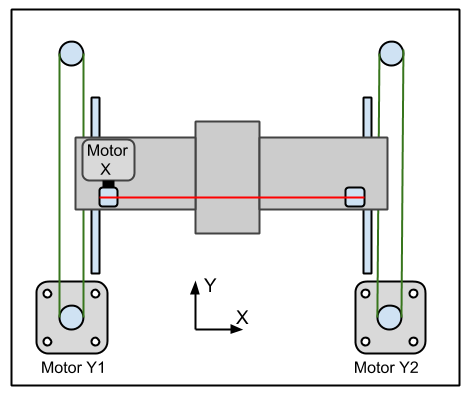
\includegraphics[width=0.6\linewidth]{obrazky/XY.png}%
    \caption{XY.}
    \label{fig:XY}
\end{figure}


V případě použití jendnoho motoru pro osu Y by bylo nutné spřažení pravé a levé části portálu, aby nedocházelo k nežádoucí rotaci při hnaní jen jedné části portálu. Alternativou by bylo na každou stranu portálu dát jeden motor a jejich otáčky řídit synchroně. 
Osa X by měla po boku vlastní motor a celá by byla uložená na ose Y. Tzn s pohybem v ose Y by se pohybovala i celá váha osy X. Na ose X je navíc ještě umístěna osa Z s vakuovou pipetou což je další hmota navíc. Dá se očekávat, že dynamické vlastnosti, rychlost a kompaktnost tohoto řešení nebude pro osazovací automat ideální (za předpokladu použití dostupných komponent).





\subsection{H-Bot}
Zajímavým uspořádáním, které úplně eliminuje nutnost aby se motor X pohyboval s osou Y z předchozího uspořádání je systém H-bot. V tomto řešení jsou motory staticky připevněné k rámu a řemen je uspořádán do tvaru H, proto H-bot. Hmota motorů se tak již nepohybuje s pohybem os, tudíž celá sestava bude mít menší setrvačnost a lze tak dosáhnout rychlých akcelerací a vysokých rychlostí. Systém využívá dva motory, kde pro pohyb mechanismu jen v jedné ose je zapotřebí obou motorů. Pokud se motory točí stejným směrem, pohybují s jednou osou. Pro pohyb v druhé ose se točí v protifázi.





\subsection{CoreXY}
Výše zmíněné nevýhoda systému H-bot jde eliminovat podobným, avšak mírně komplikovanějším uspořádáním zvaným coreXY. 

\begin{figure}[h!]
  \centering
    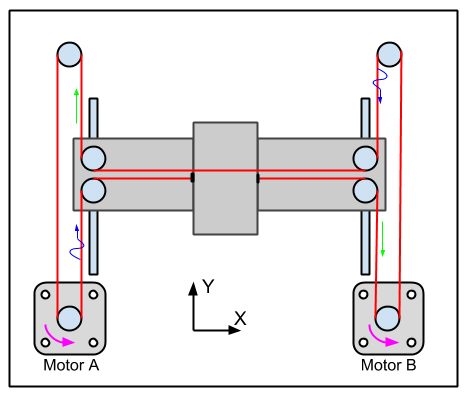
\includegraphics[width=0.6\linewidth]{obrazky/Hbot.png}%
    \caption{H-bot.}
    \label{fig:Hbot}
\end{figure}

Nevýhodou tohoto uspořádání je fakt, že síly působící na pohyblivý portál jsou v opačném směru což může vést k jeho mírné rotaci. Na obrázku je naznačen pohyb v pozitivním směru osy X, motor A i motor B se točí na stejnou stranu. Do obrázku byly naznačeny tahové a tlakové síly (zelená a modrá šipka), které by se měli v ideálním případě navzájem vyrušit. V reálném světě tomu tak není a portál má tendenci rotovat ve směru zelených šipek.
 S tímto systémem se tak dá dosahovat precizního polohování jen za předpokladu použití dostatečně tuhé konstrukce.





\subsection{CoreXY}
Výše zmíněné nevýhoda systému H-bot jde eliminovat podobným, avšak mírně komplikovanějším uspořádáním zvaným coreXY. 

\begin{figure}[h!]
  \centering
    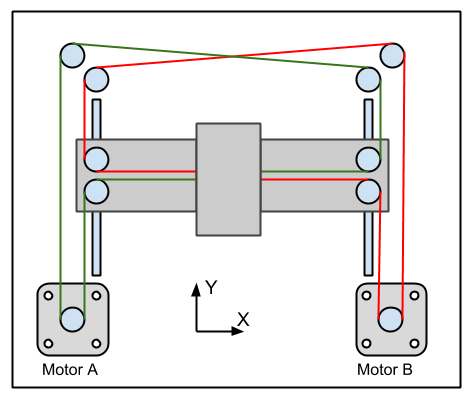
\includegraphics[width=0.6\linewidth]{obrazky/coreXY.png}%
    \caption{Core XY.}
    \label{fig:coreXY}
\end{figure}

Jak je vidět z obrázku, síly působící na portál působí oproti H bot již v jednom směru a nedochází tak k nechtěné rotaci portálu. 



%% Vložení souboru 'text/vacuum' s popisem reseni práce
\chapter{Vakuum}

Pro přemisťování součástek mezi zásobníkem a DPS je použita vakuová pipeta. Principielně pipeta najede nad součástku v zásobníku, zapne se odčerpávání vzduchu a součástka je nasáta na trysku. Po té přístroj s nasátou součástkou odjede na danou pozici DPS. Tam pipeta sjede v ose Z přímo nad DPS a vypne se odčerpávání – součástka se uvolní z trysky. V tomto stádiu je součástka osazena a celý proces se může opakovat.

Pro osazovací automat je základním požadavek na zdroj vakua bezolejový provoz. V případě použití bežně dostupných olejových rotačních pump hrozí riziko kontaminace součástek a DPS olejovými parami. Mohlo by tak dojít ke snížení pájitelnosti. Komerčně dostupnou variantou bezolejových – suchýh pump jsou Scrool pumpy a membránové pumpy. Jejich pořizovací cena je sice vyšší, ale odpadá problém s možnou kontaminací součástek.

\begin{figure}[h!]
  \centering
    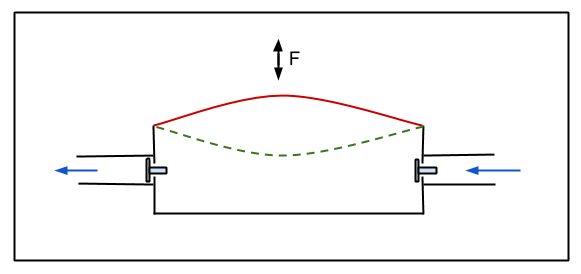
\includegraphics[width=0.6\linewidth]{obrazky/membrane.png}%
    \caption{Princip membránové pumpy.}
    \label{fig:membranka}
\end{figure}

Pro použití v osazovacím automatu byla zvolena právě membránová pumpa. Její výhodou je také minimální hlučnost. Pro srovnání u membránové pumpy Pfeiffer MVP 020-3 výrobce uvádí hlučnost $\leq$ 48 dB. Rotační pumpa Pfeiffer Hena 25 se srovnatelnou čerpací rychlostí má pak hlučnost $\leq$60 dB \cite{pfeiffer}.

\begin{figure}[h!]
  \centering
    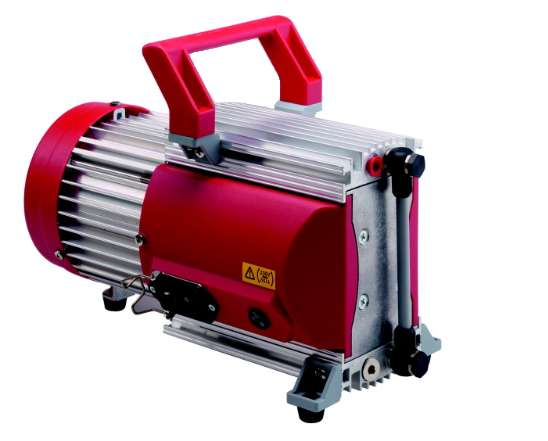
\includegraphics[width=0.6\linewidth]{obrazky/pfeiffer.jpg}%
    \caption{Membránová pumpa Pfeiffer MVP 020-3\cite{pfeiffer}.}
    \label{fig:pfeiffer}
\end{figure}



Jako efektivní způsob řízení vakua se ukázalo mít pumpu neustále zapnutou a zapínání/vypínání pipety řídit pomocí ventilu. A to hlavně z důvodu čerpací rychlostí. V případě zapínání a vypínání celé pumpy by se muselo vyčerpat celé vakuové potrubí, kdežto při použití ventilů se zčerpává jen malý oběm mezi ventilem a tryskou. Celý proces je tak i za použití pumpy s nižší čerpací rychlostí dostatečně rychlý a není tak limitním faktorem pro rychlost osazování.

S výhodou se dá mezi pumpou a ventilem použít vakuovy buffer. Pumpa ho neustále předčerpává a tvoří tak vakuovou rezervu na výkryv náhlého zvýšení tlaku po otevření ventilu. Tímto trikem se opět dosáhne mírného zrychlení k provedení jednoho cyklu.

\begin{figure}[h!]
  \centering
    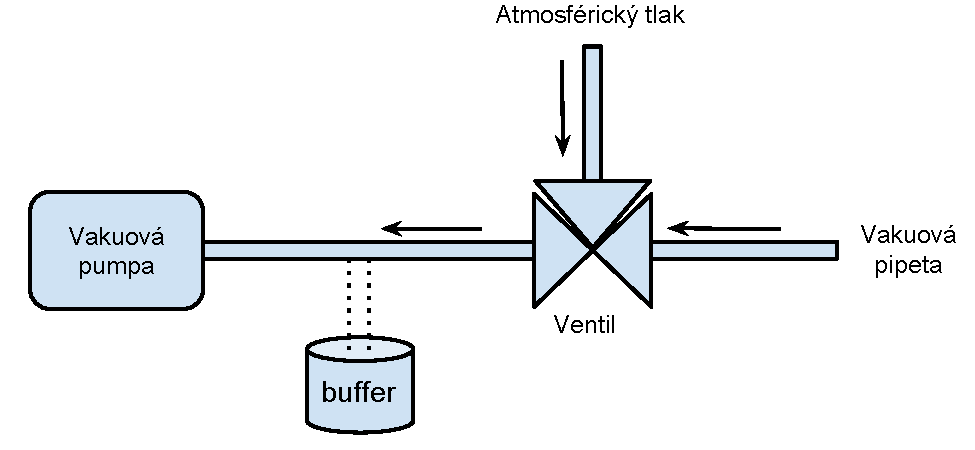
\includegraphics[width=0.8\linewidth]{pdf/vacdiagram2.pdf}%
    \caption{Uspořádání vakuové soustavy.}
    \label{fig:vacuum}
\end{figure}


S ventilem je potřeba se vypořádat s nežádoucím jevem, že součástky v operaci umisťování na DPS zůstavají přisáty na trysce i po jeho zavření. V oblasti mezi tryskou a ventilem totiž zůstává podtlak a je proto nutné ji dostat na atmosférický tlak. To se dá řešit za pomocí druhého 'napouštěcího' ventilu, který se otevře ihned po zavření ventilu od pumpy. A nebo lépe dvoucestným ventilem. Z důvodu úspory místa a zjednodušení konstrukce jsem zvolil dvoucestný ventil. Konkrétně typ V114A-5GU od firmy SMC s napájením 24V.

\begin{figure}[h!]
  \centering
    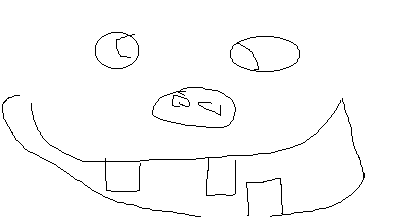
\includegraphics[width=0.3\linewidth]{obrazky/placeholder.png}%
    \caption{Vnitřní uspořádání ventilu SMC V114A.}
    \label{fig:ventil}
\end{figure}

Ventil je velice kompaktní, ale nemá možnost přímého připojení vakuového potrubí. Bylo tak nutné vyrobit rozvodný blok viz obrázek \ref{fig:ventilblok}.  Z leva je port na připojení pipety, port uprostřed je určený na připojení tlkového senzoru. Pravý port se pak připojuje k pumpě. 

\begin{figure}[h!]
  \centering
    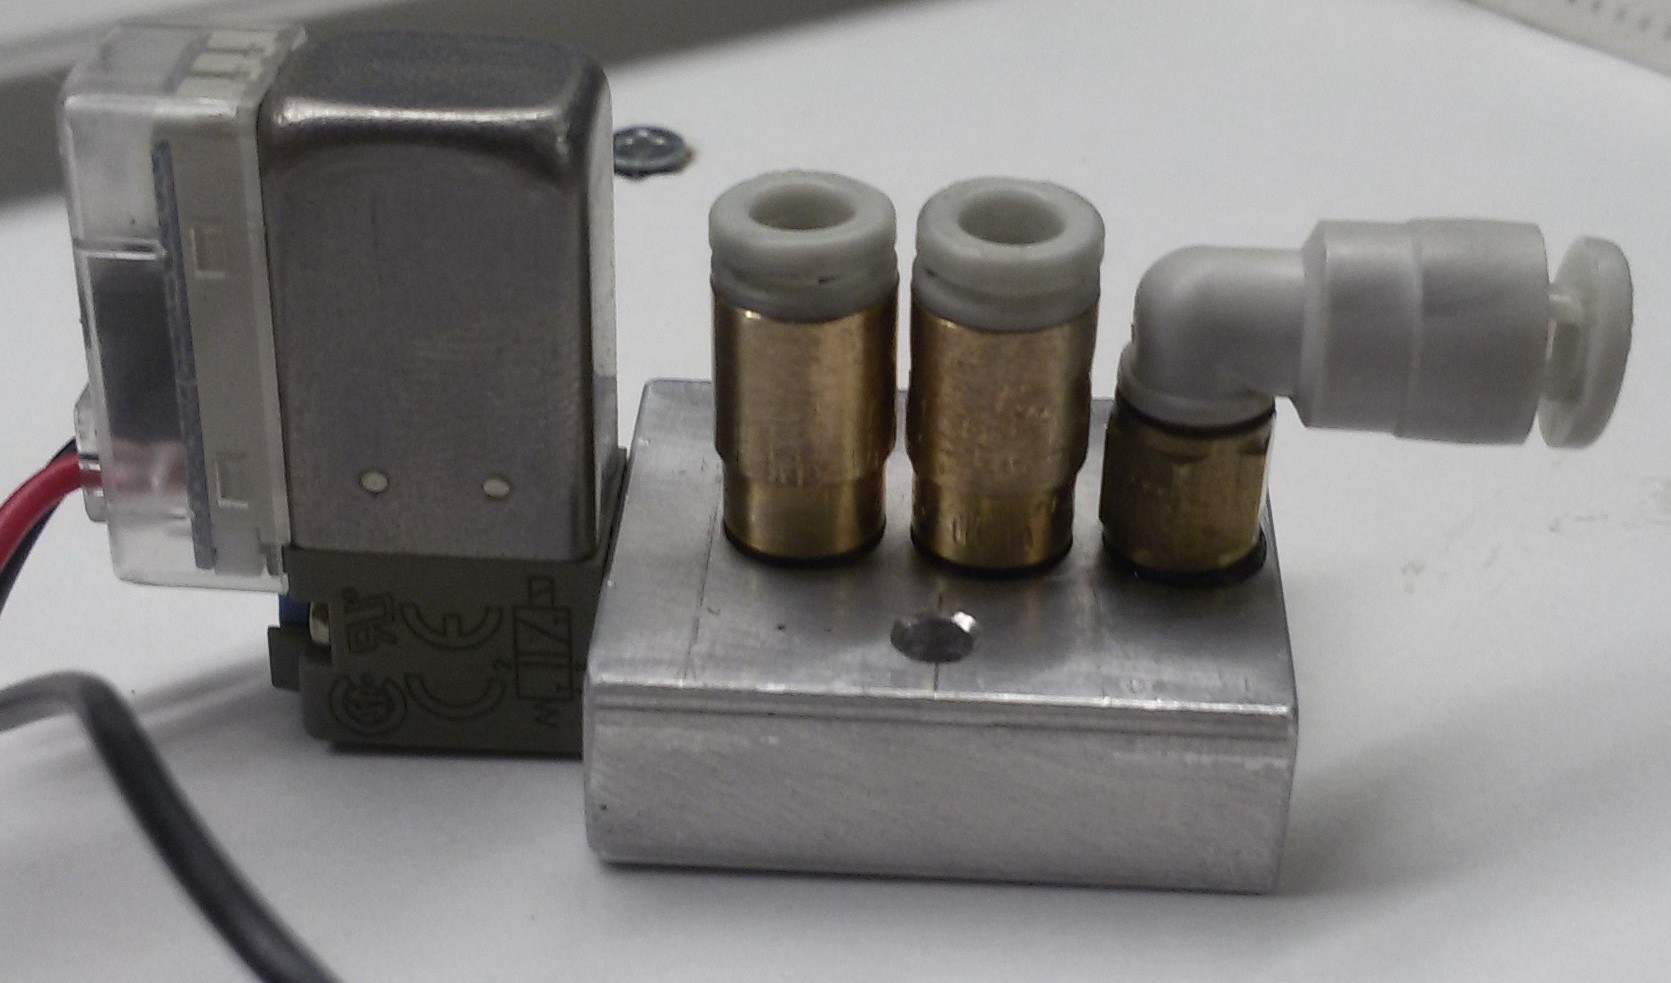
\includegraphics[width=0.7\linewidth]{obrazky/blok.jpg}%
    \caption{Rozvodný blok ventilu.}
    \label{fig:ventilblok}
\end{figure}

Vakuové porubí je z vetšiny tvořeno PTFE trubičkou s vnějším průměrem 4mm a s vnitřním 2mm. PTFE trubička je dostatečně tuhá, že u ní nedochází ke deformaci/zborcení stěn při jejím vyčeprání. Pouze na místech kde bylo potřeba malého rádiusu vedení a nebo jeho pružnosti byla použita měkčí SMC hadička z polyurethanu. K připojení potrubí posloužily rychlospojeky od SMC.

Při nasávání součástek na trysku se se může stát, že se součástku nepovede nasát. Jako jeden z kontrolních mechanismů je k vakuovému potrubí připojena tlaková sodna. Pro měření podtlaku od atmosférického tlaku se v průmyslu používají Piraniho měrky. Pro naši aplikaci ale postačí polovodičový piezorezistivní sensor v absolutní verzi. Tzn porovnávání měřeného tlaku vůči referenčnímu vakuu. 

Senzorem je potřeba detekovat následující stavy:
\begin{itemize}
\item atmosférický tlak
\item součástka přisáta na pipetě
\item součástka nepřisáta na pipetě
\end{itemize}


\begin{figure}[h!]
  \centering
    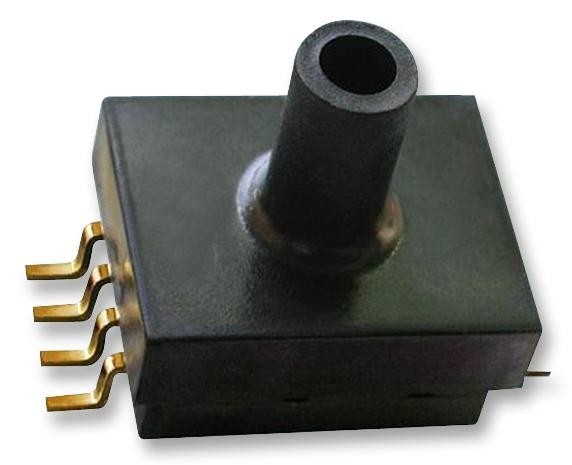
\includegraphics[width=0.4\linewidth]{obrazky/sensor.jpg}%
    \caption{Vakuový sensor  MPXM2202AS – Fotka FARNELL, nutno vyfotit vlastní.}
    \label{fig:sensor}
\end{figure}

Vybraný typ senzoru je Freescale semiconductor MPXM2202AS s rozsahem měření od 200kPa až do 0kPa.  Senzor pracuje v rozsahu napájecíh napětí 10-16V a jeho výstup je diferenciální.

Diferenciální výstup senzoru je pouhých 40mV pro celý rozsah měřených tlaků. Vybraný mikroprocesor disponuje 12 bitobvým ADC převodníkem což dává  4096 měřených úrovní. Pokud by se diferenciální napětí měřilo napřímo bez zesílení, výstup z ADC by se pohyboval pouze v rozmezí úrovní 0-50. Z toho polovina by navíc případala pro tlaky větší než atmosférické. Pokud vezmeme v potaz i šum, tak takovéto rozlišení není dostačující.

Finální podoba  řídícího obvodu se tak skládá z lineárního stabilizítoru 7812 a diferenciálního zesilovače. Při atmosférickém tlaku byl výstup zesilovače nastaven pomocí trimru Rxxx na 3V. Se snižujícím se tlakem se výstupní napětí také snižuje.

 Senzor i s řídící elektronikou je umístěn přímo u vakuové pipety. Signálový kabel tak povede v kabelové šachtě zároveň s kabely pro Z a R motory. Z obavy, že by se na výstupním analogovém signálu mohlo indukovat rušivé napětí je řídící obvod vybaven i komparátorem, který bude mikrosprocesoru sinalizovat log 1, nebo 0 dle přítomnosti atmosféry, nebo vakua. Snahou ale bylo, aby šel analogový výstup připojit přímo na ADC mikroprocesoru, což se povedlo.


\section{Diferenciální zesilovač - TODO}

\section{Měření výstupu z ADC}
Bylo zapotřebí vhodně zvolit prahové hodnoty ADC pro rozlišení jednotlivých detekovaných stavů. Proto byla provedena série měření. Předpokladem bylo, že nejhorší rozlišovací schopnost bude v případě trysky nejmenšího průměru (0,5mm), kde rozdíl v tlacích mezi stavy součástka přítomna/nepřítomna bude minimální. To se i potvrdilo, viz následující graf.

\begin{figure}[h!]
  \centering
    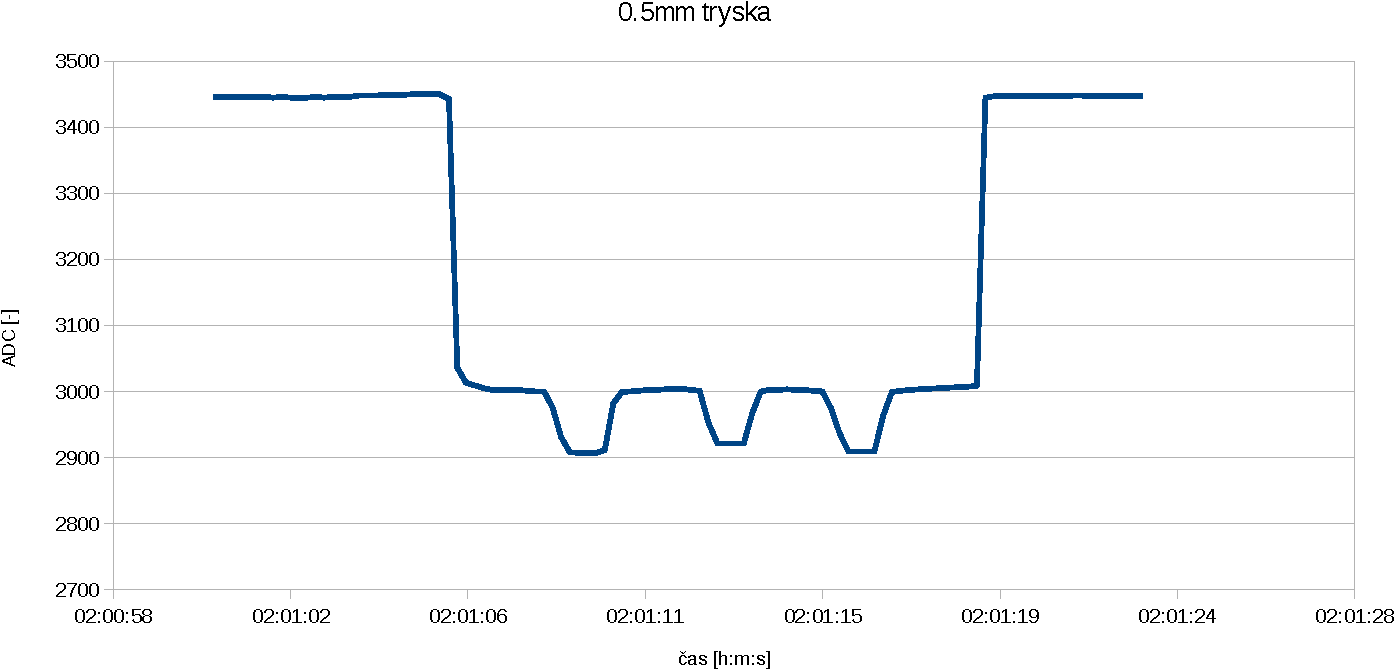
\includegraphics[width=0.9\linewidth]{pdf/5mm-crop2.pdf}%
    \caption{0,5mm tryska.}
    \label{fig:sensor}
\end{figure}

Rozdíl ve výstupu ADC mezi stavem součáskta přítomna/nepřítomna je přibližně 100.

Jelikož osazovací automat má výměnné trysky, byl stejný test proveden i pro trysku o průměru 0,9mm. V tomto případě byl rozdíl mezi stavy součáskta přítomna/nepřítomna mnohem markantnější – 400.

\begin{figure}[h!]
  \centering
    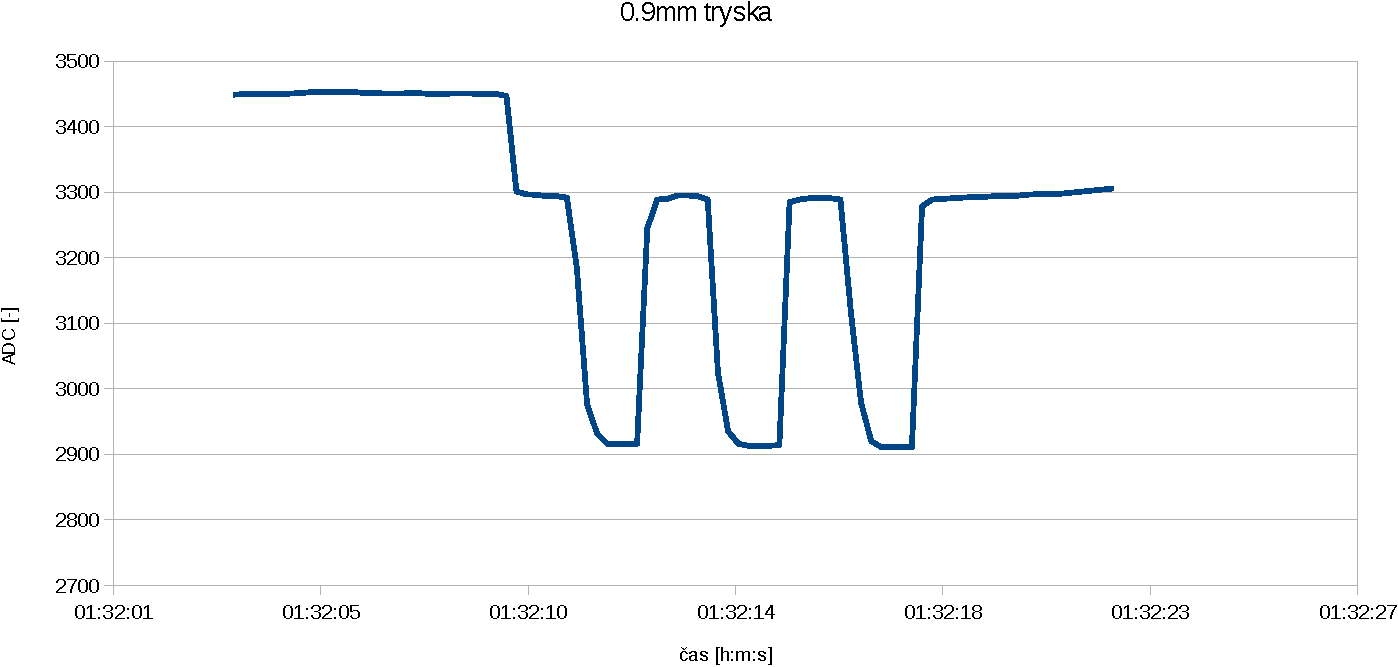
\includegraphics[width=0.9\linewidth]{pdf/9mm-crop2.pdf}%
    \caption{0,9mm tryska.}
    \label{fig:sensor}
\end{figure}


Rozlišovací hodnoty ADC pro jednotlivé stavy byly na základě měření stanoveny následnovně.
Atmosféra – 4096 až 3350
Součástka nepřítomna 3550 až 2950
Součástka přítomna 2950 až 0
Tyto hodnoty byly náseldně implementovýny do řídícího SW.


\section{Vakuová pipeta a tryska}
Sestava vakuové pipety musí být schopna pro vyzvednutí součástek motorizovaného pohybu v ose Z. Rozsah pohybu v ose Z je dán minimálně dvojnásobkem výšky nejvyšší osazované součástky. Dle tabulky \ref{table:pasky} je maximální výška součástek pro 24mm pásku 11.9mm. Minimální rozsah osy tak vychází na 23.8mm. Dále je před osazením potřeba nasáté součástky na pipetě narotovat do požadované rotace. Proto musí být pipeta motorizováná i v ose R. Oba tyto požadavky komplikují vedení vakuového potrubí.

\subsection{Tryska}
Použití komerčně dostupné varianty trysek pro osazovací automaty nebylo pro svoji cenu a složitost adaptace uvažováno. Jako alternativa posloužily upravené injekční jehly k injekčním stříkačkám. Jehly jsou dostupné v širokém rozpětí průměrů, což je ideální pro možnost přizpůsobení velikosti trysky k dané osazované součástce. Samotnou jehlu bylo pootřeba vhodným způsobem připevnit ke hřídeli rotačního motoru. S tím také vyvstala otázka jak řešit připojení vakuového potrubí. 
Jedním z požadavků zadání diplomové práce byla možnost manuální výměny trysky/pipety. Bylo tedy zapotřebí vytvořit adaptér mezi jehlou a motorem, ke kterému se připojí vakuové potrubí.


\begin{figure}[H]
  \centering
    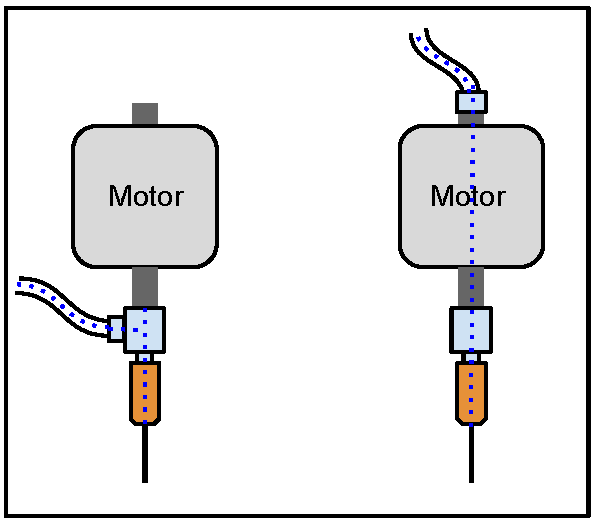
\includegraphics[width=0.6\linewidth]{pdf/motorR2.pdf}%
    \caption{Obrázek možných řešení vakuového vedení. Pro názornost byla modrým tečkováním naznačena cesta vakuového potrubí.}
    \label{fig:sensor}
\end{figure}

Jak se ale při praktických experimentech ukázalo, tak z hlediska vyhodnocování obrazu je žádoucí mít při pohledu spodní kamerou okolo součástky uniformní pozadí. Řešení pomocí bočně připojeného potrubí tak bylo zavrženo. 
Namísto toho byl použit pro osu R motor s dutou hřídelí, která byla použita jako vakuové vedení. Toto řešení umožnilo získávat ze spodní kamery snímky s uniformním pozadím. 

Vysoustružená mosazná redukce byla k hřídeli připevněna pomocí stavěcích šroubů a zatěsněna dvousložkovým lepidlem Torrseal, který je určen do aplikací vyžadujících vakuovou těsost.
Jak zadání práce vyžadovalo, vznikla tak funkční sestava s možností manuální výměny trysky.

\begin{figure}[h!]
  \centering
    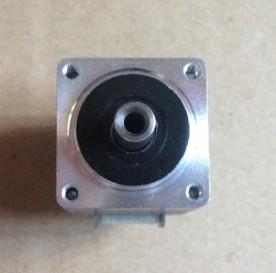
\includegraphics[width=0.6\linewidth]{obrazky/robotdigg_nema8.jpg}%
    \caption{Ukázka použitého motoru Nema8 s dutou hřídelí.}
    \label{fig:nema8}
\end{figure}

\begin{figure}[h!]
  \centering
    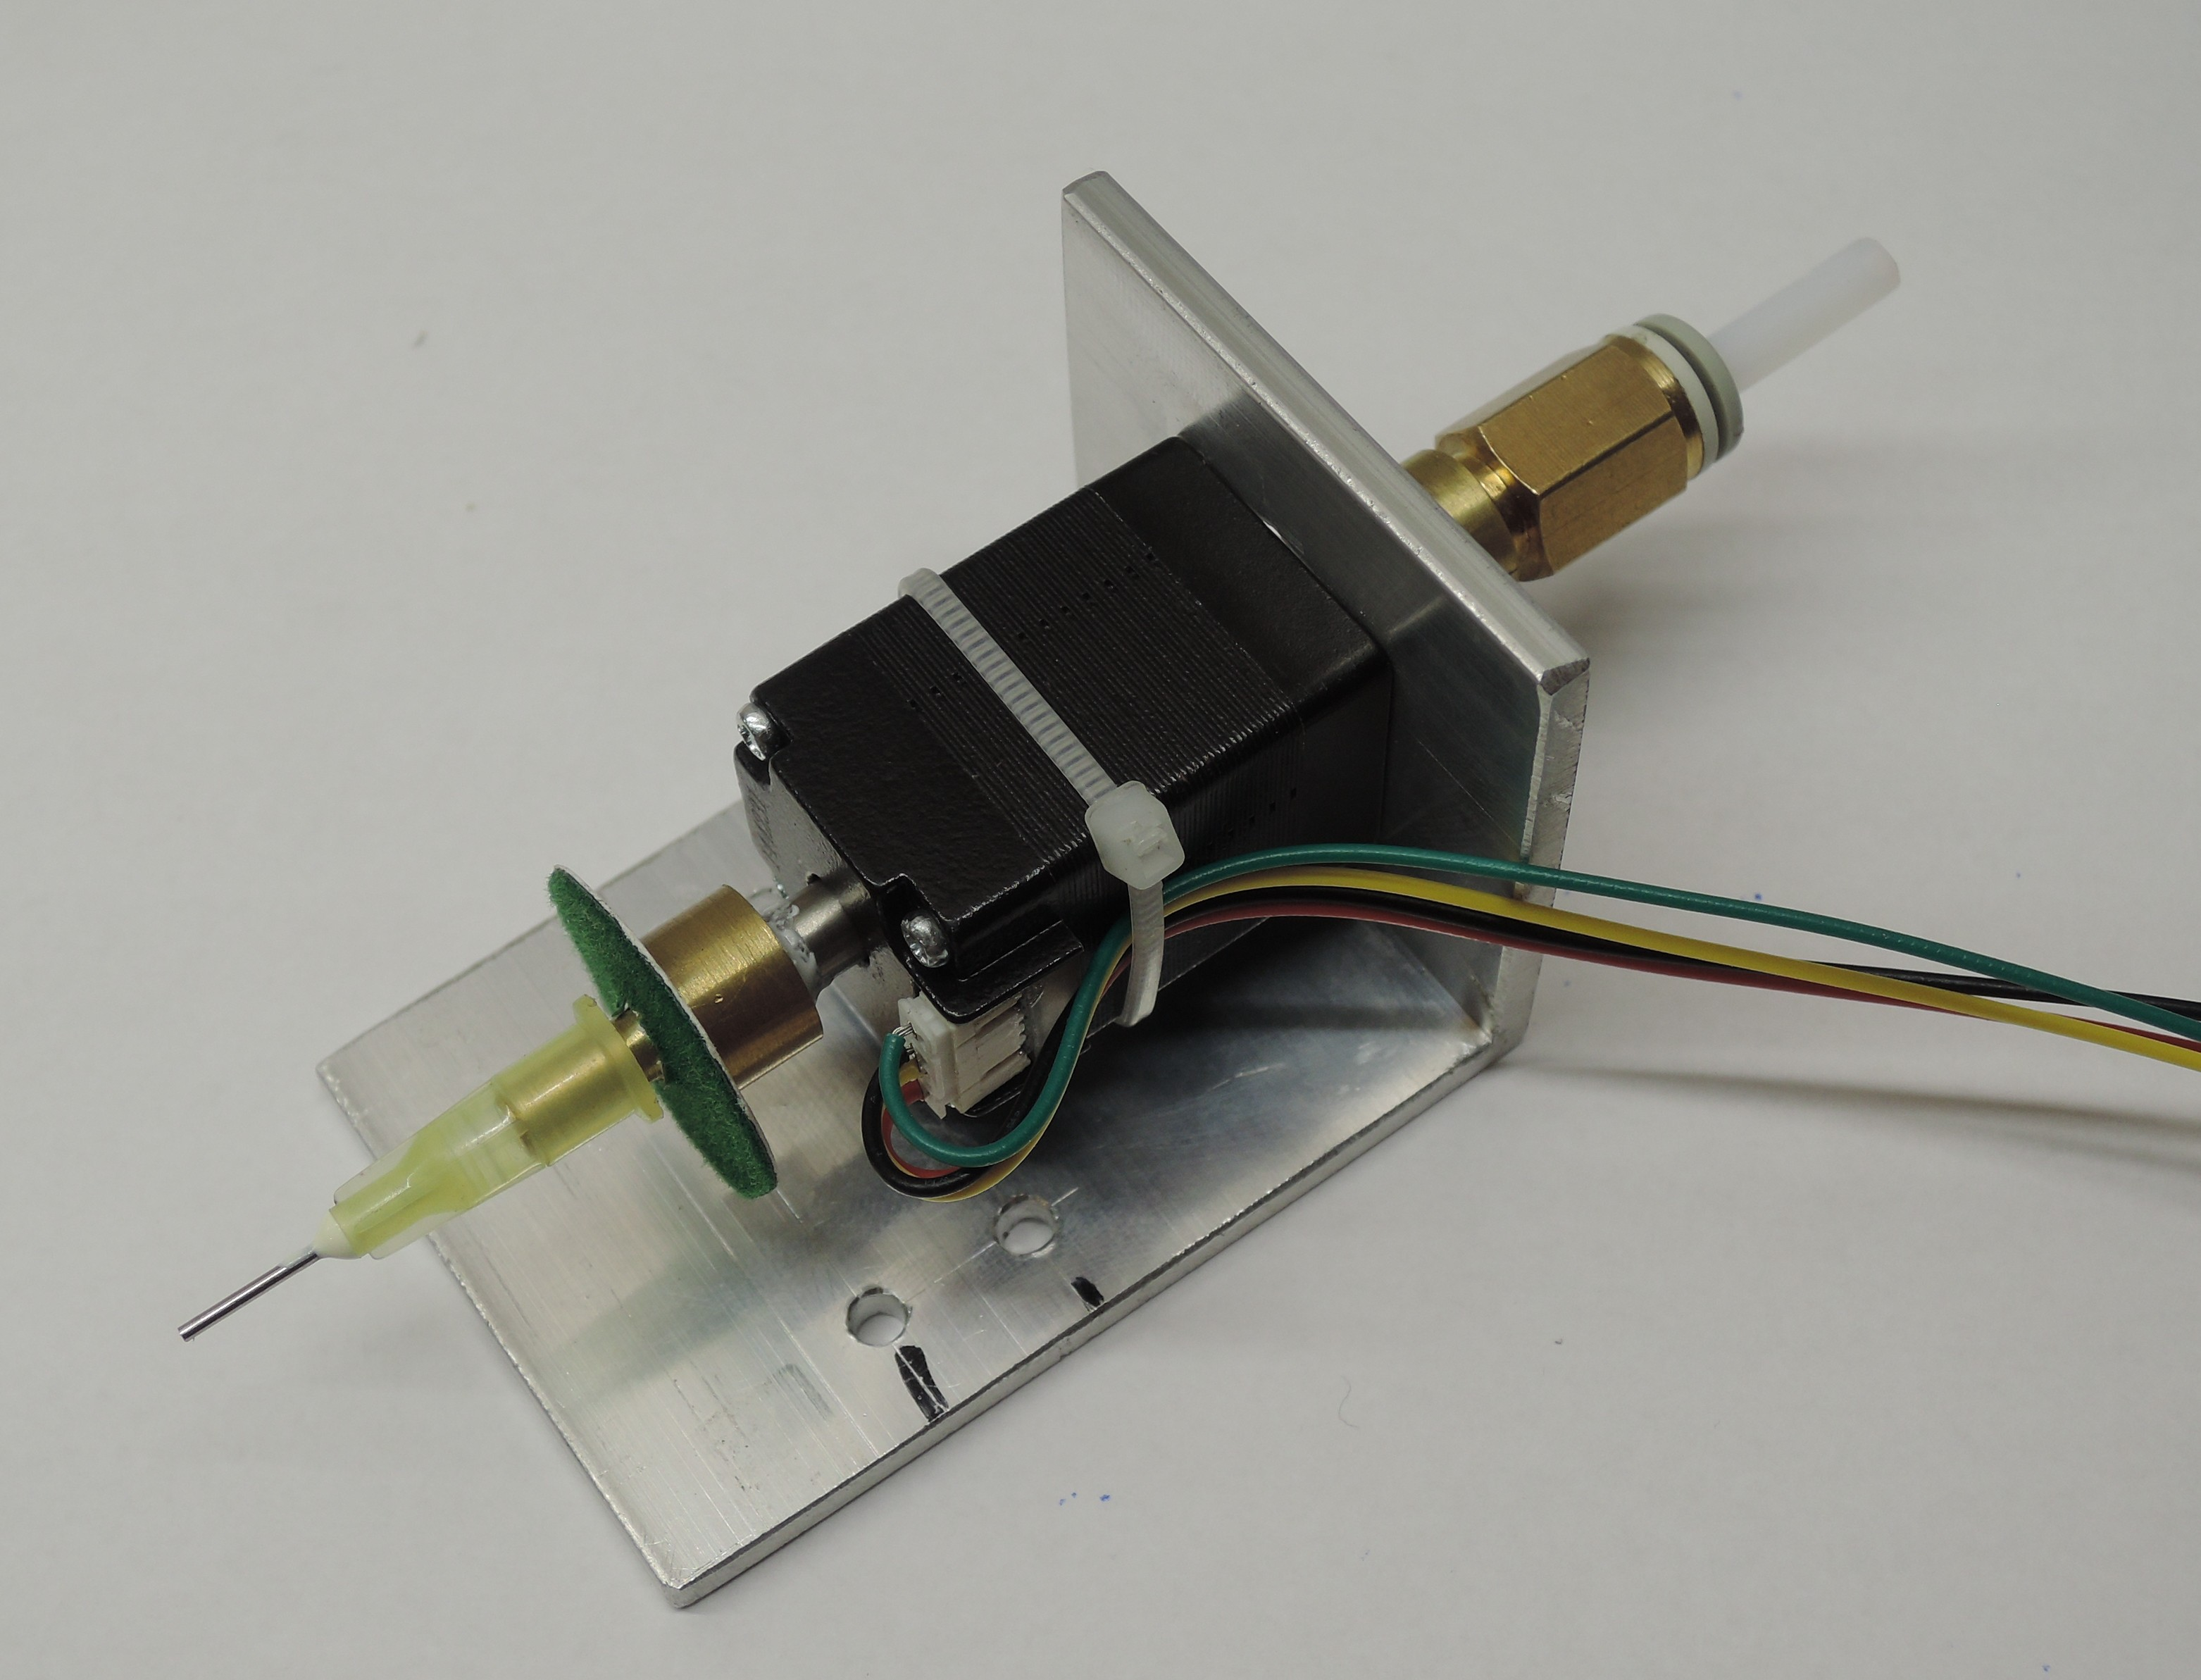
\includegraphics[width=0.8\linewidth]{obrazky/tryska2.jpg}%
    \caption{Detail vysoustružené redukce s nasazenou 0.9 mm tryskou.}
    \label{fig:tryska}
\end{figure}




%% Vložení souboru 'text/reseni' s popisem reseni práce
\chapter{Vyhodnocování obrazu}




%% Vložení souboru 'text/elektro' s popisem vysledků práce
\chapter{Řídící elektronika}

Řídící elektronika osazovacího automatu má za úkol obstarávat následující funkce:
\begin{itemize}
\item komunikace s počítačem přes USB rozhraní
\item řízení motorů pro osy X, Y, Z, R (rotace)
\item řízení a měření vakua
\end{itemize}


Elektronika je založena na mikrokontroléru LPC1769 od firmy NXP. Je to moderní 32-bitový mikrokontrolér bežící na frekvenci 120 MHz s celou řadou integrovaných funkcí jako USB, ADC, DAC, UART a další. Jádrem mikrokontroléru je ARM\textregistered Cortex\textregistered-M3.

Mikrokontrolér komunikuje s řídícím SW přes USB rozhraní. Obstarává veškerou režii řízení krokových motorů a zároveň řídí všechny vstupně výstupní periferie. Blokový diagram je znázorněn na obrázku \ref{fig:ridici}, jednotlivé bloky jsou pak popsány v následujících podkapitolách.

\begin{figure}[h!]

  \centering
    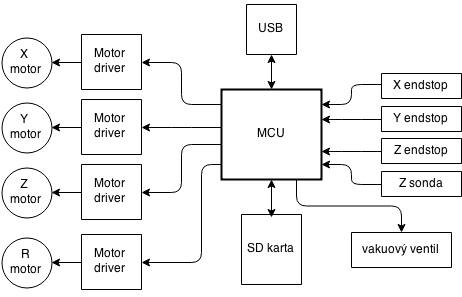
\includegraphics[width=0.8\linewidth]{obrazky/electronics.png}%
    \caption{Diagram řídící elektroniky.}
    \label{fig:ridici}
\end{figure}


\section{Firmware}

Firmware slouží jako mezičlánek mezi PC a hardwarem osazovacího automatu. Přijmá příkazy od řídícího SW a ty pak vykonává.

Ověřeným standardem pro instruování CNC strojů jsou tzv G-kódy. Programovací jazyk G, specifikován pod standardem RS274D umožňuje pomocí jednoduchých instrukcí řízení celého stroje. Bohužel standard RS274D ale není striktně dodržován a výrobci CNC strojů a řídících kontrolérů si upravují a vytváří vlastní specifické G-kódy.

Struktura G-kódu je následující: {\bf G}<číslo> <parametry>.\\
Pomocí {\bf G}<číslo> se rozlišuje o jaký příkaz se jedná a <parametry> jsou vstupní parametry příkazu. Jako ukázka poslouží kód na pohyb v osách {\bf G0}, ten bere parametry název osy a cílovou pozici osy.
\begin{verbatim}
  G0 X-10.3 Z12
\end{verbatim}

Parametry X-10.3 a Z12 tedy udávají, jaké osy a kam se mají pohnout. Není však specifikováno, jestli se jedná o absolutní, nebo relativní pohyb. K tomu slouží příkazy {\bf G90} (absolutní) a {\bf G91}(relativní) pohyb.
Všechny příkazy jsou vykonávány v posloupnosti tak, jak je mikrokontrolér obdrží. Následující posloupnost příkazů tedy nastaví stroj z počáteční pozice na pozici X0, Y10, Z0,4, poté provede relativní pohyb X5, Z2. Výsledná pozice stroje je tedy X5, Y12, Z0,4.

\begin{verbatim}
  G90
  G0 X0 Y10 Z=0.4
  G91
  G0 X5 Z2
\end{verbatim}

Obdobou G příkazů jsou M příkazy, které slouží na vykonávání příkazů přímo nesuvisejících s pohybem stroje. Pro příklad příkaz {\bf M42} slouží ke spínání vakuového ventilu.

Z důvodu komplexnosti celé diplomové práce by bylo napsání kvalitního firmware příliš časově náročné. Proto byl jako základ použit firmware Smoothie od autora Arthura Wolfa napsaný v programovacím jazyku C++. Pro uzpůsobení firmware pro osazovací automat bylo potřeba provést celou řadu úprav. Ne všechny požadované funkce byly totiž ve firmware dostupné. Chyběla hlavně podpora tlakového senzoru.
Zajímavou funkcí firmware je možnost jeho konfigurace přes textový soubor uložený na SD kartě. Ke každému pinu mikrokontroléru lze v konfiguračním souboru přiřadit libovolnou funkcu. 
Jako ukázka je uvedena konfigurace motoru k ose X. K pinu 0 na portu 2 mikrokontroléru byl přiřazen signál step (krok) motoru. Ovládání směru otáčení je na pinu 5 port 0, kde vykřičník znamená invertování směru otáčení. K portu 1 pinu 4 je nakonec přiřazen signál enable, který aktivuje motor.
\begin{verbatim}
  alpha_step_pin	2.0
  alpha_dir_pin		0.5!
  alpha_en_pin		1.4
\end{verbatim}


Protože firmware čte konfigurační soubor z SD karty, bylo zapotřebí ošetřit možnost zapnutí řídící elektroniky bez zasunute karty. Pokud by taková situace nastala, jednotlivé piny by byly v nedefinovaném stavu a mohlo by dojít k poškození osazovacího automatu. Proto byla ve firmware ke každnému použitému pinu přiřazena defaultní hodnota. Tato hodnota se dá později pomocí konfiguračního souboru změnit.
\\

Kompletní firmware s doprogramovanými funkcemi lze najít v příloze C. Jedná se již o zkompilovaný firmware ve formátu .bin  Z důvodu nadměrné velikosti nejsou zdrojové soubory součástí přílohy. Aktuální verzi zdrojových kódů modifikovaného firmware je ale možné získat přes internet za pomocí programu GIT příkazem:
\begin{verbatim}
  git clone https://github.com/Hyna/Smoothieware.git
\end{verbatim}
	




\section{Krokové motory a jejich drivery}

Horní a spodní kamera se připojuje přes USB rozhraní přímo do počítače nezávisle.

Jelikož je osazovací automat koncipován spíše na prototypovou výrobu, případně na první série DPS, není rychlost osazování kritická. I přesto byl ale kladen důraz na dosažení co největší osazovací rychlosti.

Jako vhodný typ motorů připadaly v úvahu krokové motory a servo motory. Servo motory by dozajista byly lepší volbou pro svůj velký kroutící moment a uzavřenou smyčku řízení. Oproti krokovým motorům jsou ale náročnější na řízení a mají vyšší cenu.
Volba tak padla na krokové motory u kterých je řízení jednodušší. Za použití driveru je lze ovládat jen pomocí signálu Krok a Směr (STEP a DIRECTION). Řízení je pak otevřenou smyčkou, krokový motor nemá žádnou zpětnou vazbu.

Může řídit jen jen zátěž, která je v rozsahun na kterou byl dimenzován. V opačném případě dochází ke ztrátě kroku a tím i pozice.

U krokového motoru se vzrůstající rychlostí rotace klesá kroutící moment. Od jakých otáček dochází k poklesu je ale zavislé na napájecím napětí. To je názorně vidět na momentové charakteristice pro motor SX17-1005LQEF od české firmy Microcon. Právě tento motor byl do konstrukce použit.


\begin{table}[h!]
  \caption{Katalogové parametry motoru SX17-1005LQEF }
  \begin{center}
  	\small
	  \begin{tabular}{|c|c|c|c|}
	    \hline
	    Statický moment [Nm]		& Příruba 		& Jmenovitý proud [A]	& Krok [°]	\\
	    \hline\hline

		0,51				& Nema 17		& 1,0			& 1.8		\\

	    \hline
	  \end{tabular}
  \end{center}
\end{table}

Konečná volba napájecího napětí byla dána s ohledem na vakuové ventily. Ty potřebují pro spolehlivý provoz napájení 24V, viz kapitola Vakuum. Celé zařízení tedy bude používat jednotné napájení 24V, aby odpadla nutnost mít dva různé napájecí zdroje.


Pro řízení motorů byl použit Pololu driver s integrovaným obvodem DRV8825 od Texas instruments. Driver je schpný bez aktivního chlazení do motoru dodávat až 1.5A při napájecím napětí do 45V. Plně tak vyhovuje pro použití s vybraným typem motoru SX17-1005. Navíc disponuje variabilně nastavitelným mikrokrokováním os 1/2 až do 1/32. 
Zvolený motor má krok 1.8° což odpovídá 200 krokům na otáčku. Na volbě mikrokroků tak bude záviset teoretická přesnost pozicování.

\begin{figure}[h!]

  \centering
    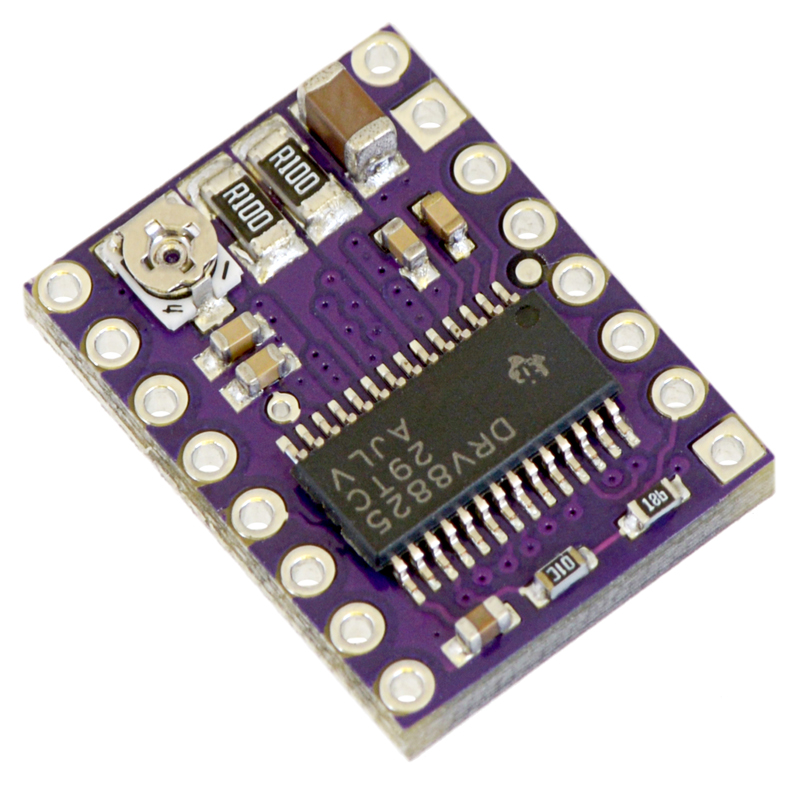
\includegraphics[width=0.4\linewidth]{obrazky/DRV8825.jpg}%
    \caption{DRV8825.}
\end{figure}

Jednoduchým výpočtem pak zjistíme, kolik kroků bude potřeba pro pohyb dané osy na jeden mm a teoretickou přesnost pozicování. Parametry kroky/mm je později použit na klaibraci os.
 
Použitý řemen GT2 má rozteč 2mm a řemenice má 20 zubů – viz kapitola o mechanické konstukci.
Krok na mm = (kroků na otáčku * mikrokroky) / (rozteč zubů řemenu  * počet zubů řemenice)
přesnost pozicování se pak vypočte jako převrácená hodnota počtu kroků na mm.

\begin{table}[h!]
  \caption{Mikrokrokování }
  \begin{center}
  	\small
	  \begin{tabular}{|c|c|c|}
	    \hline
	    Mikrokrokování		& Kroků na mm 		& Přestnost pozicování [um] 	\\
	    \hline\hline

		1 – celý krok 		& 5			& 200 				\\
		\hline
		1/2			& 10			& 100				\\
		\hline
		1/4			& 20			& 50				\\
		\hline
		1/8			& 40			& 25				\\
		\hline
		1/16			& 80			& 12,5				\\
		\hline
		1/32			& 160			& {\bf 6.25} 			\\
		\hline
	    \hline
	  \end{tabular}
  \end{center}
\end{table}

Jak vyplývá z tabulky, pro režim mikrokrokování 1/32 vychází teoretická přesnost 6,25 um. Co nejpřesnější pozicování je při osazování součástek žádoucí, proto byl driver nakonfigurován do tohoto režimu pomocí jumperů na konektoru MS4. Pro režim  1/32 se signály MS1, MS2 a MS3 připojují na Log 1.   Driver je ovládán signály EN – aktivace driveru, STEP - krok a DIR – směr přímo z procesoru. Konektor M4 pak slouží pro připojení krokového motoru. Význam a konfiguraci dalších pinů driveru lze najít v datasheetu.

\begin{figure}[h!]

  \centering
    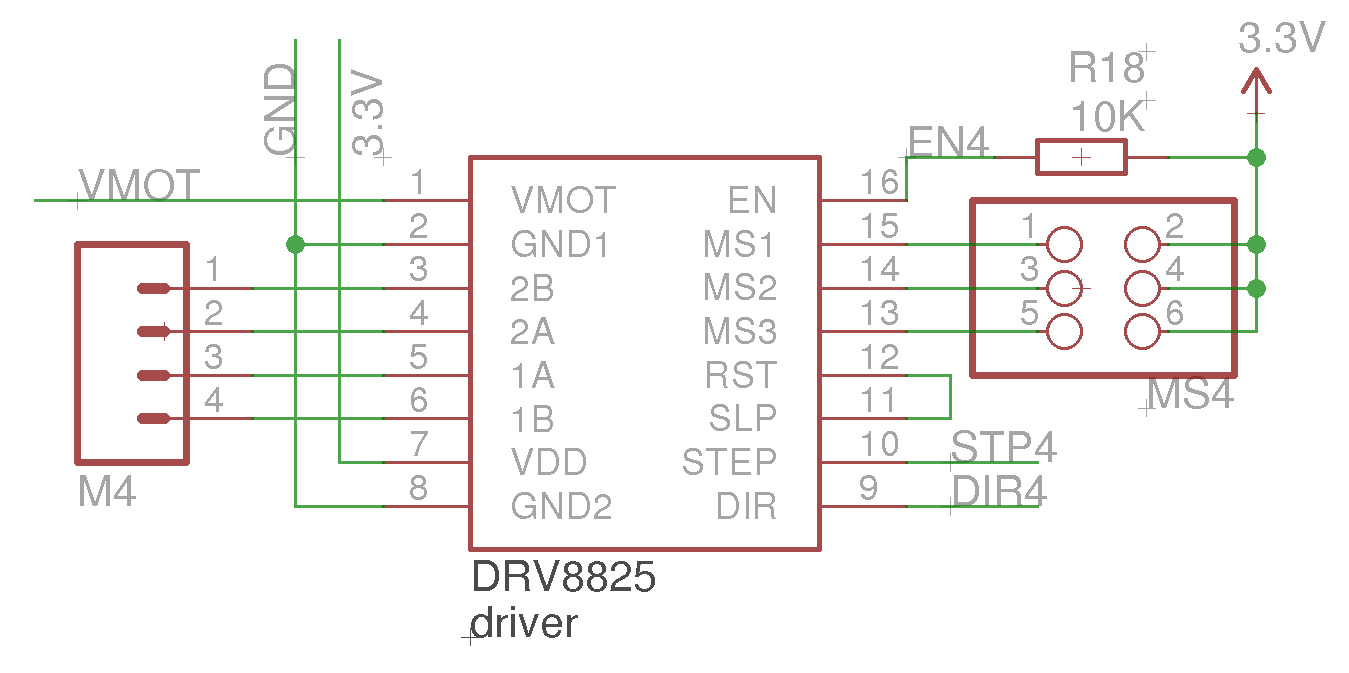
\includegraphics[width=0.8\linewidth]{obrazky/motorDriver.png}%
    \caption{DRV8825.}
\end{figure}

\begin{figure}[h!]

  \centering
    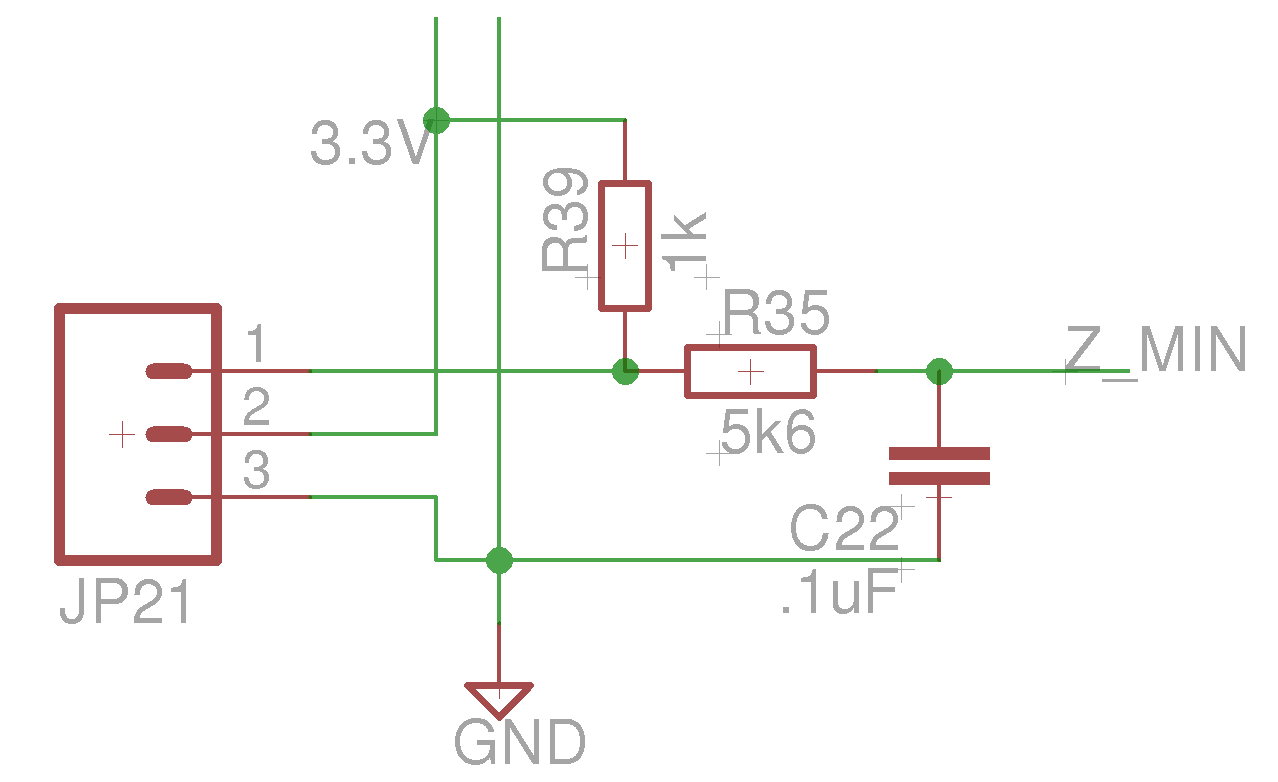
\includegraphics[width=0.6\linewidth]{obrazky/endstops.png}%
    \caption{Koncové dorazy.}
\end{figure}



\section{USB a elektromagnetická kompatibilita}

Mikrokontrolér disponuje nativní podporu USB protokolu verze 2.0, nebylo tak nutno žádných externích převodníků. Zapojení vychází z katalogového doporučení od výrobce mikrokontroléru. Odpory R8 a R9 na impedanční přizpůsobení, kondenzátory C4 a C5 na potlačení rušivých vysokofrekvenčních sgnálů.

\begin{figure}[h!]

  \centering
    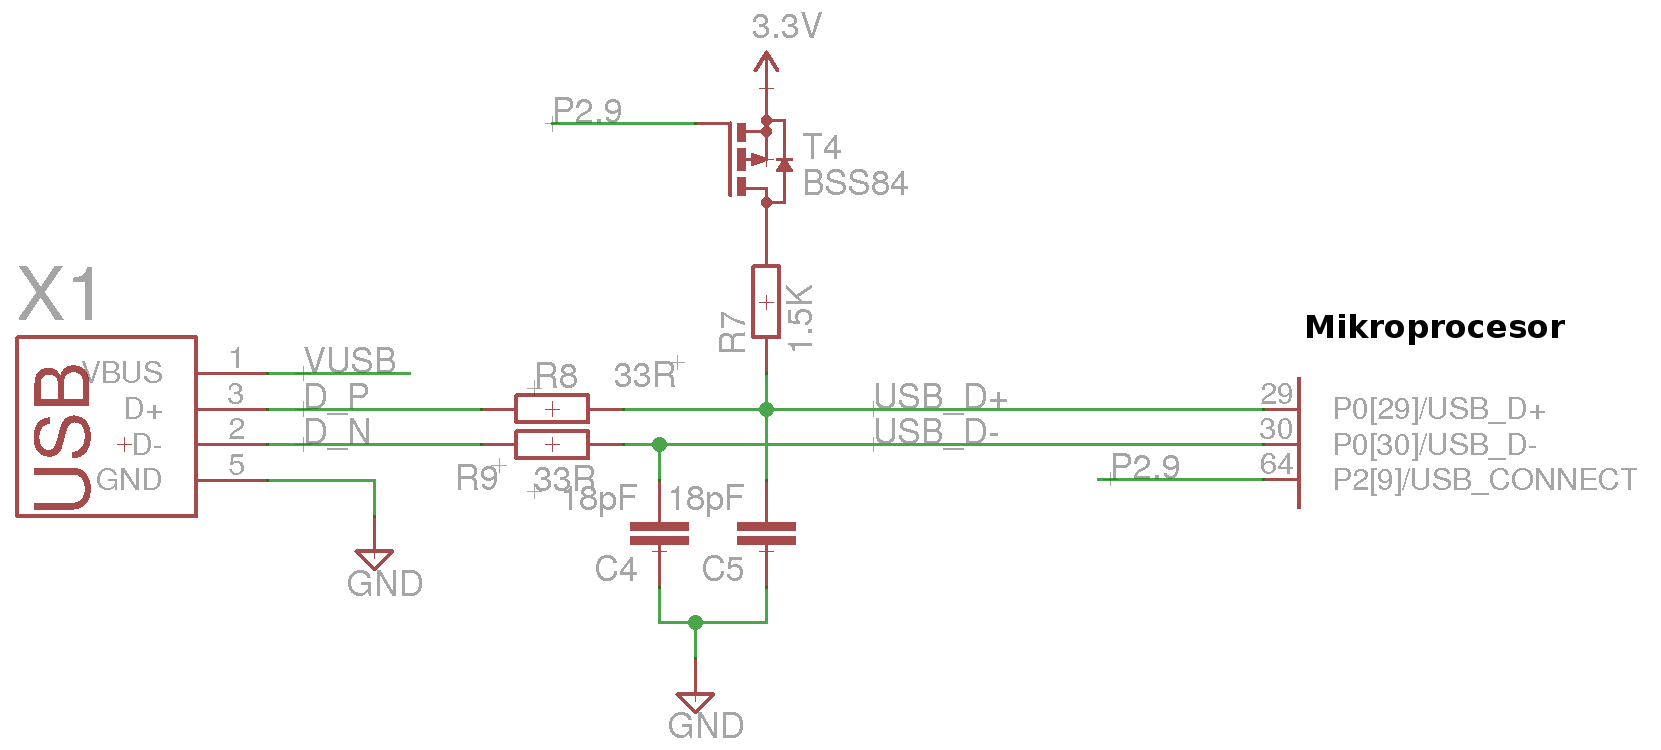
\includegraphics[width=0.8\linewidth]{obrazky/usb.png}%
    \caption{Zapojení USB.}
\end{figure}

Na následujícím obrázku je vidět původní zapojení prototypu řídící elektroniky. Jak bylo řečeno, vychází z doporučeného zapojení od výrobce a bylo navíc doplněno o kondenzátory C4 a C5 pro potlačení rušení dle \cite{intel}. V průběhu testování a psaní řídícího SW se ale bez zjevné příčiny stávalo, že došlo k přerušení komunikace s mikrokontrolérem. První podezření bylo na zamrzající (je to spisovný?) firmware mikrokontroléru a jeho reset. Pro ověření této doměnky byl k desce připojen externí převodník USB na sériové rozhraní. Po zamrznutí USB rozhraní se ale dalo stále připojit externím převodníkem a komunikovat s mikrokontrolérem. Problém tedy byl jen se samotným nativním USB rozhraním. 
První podezření na elektromagnetickou kmpatibilitu nastalo až při zapojování vakuové pumpy do rozvodné sítě. Deska reprodukovatelně přestávala komunikovat přes USB rozhraní. Měřením na osciloskopu se neprokázalo, že by se rušení šířilo vedením – napájecími kabely. 
Jednalo se tedy o rušení indukované. Za použití nacvakávacích feritů byl identifikován jako hlavní zdroj rušení USB kabel. Při používání feritů je důležité umisťovat je co nejblíže koncům kabelů.
Použitý propojovací USB kabel byl značky Goobay od Německého dodavatel a disponoval značkou CE. Rovněž použití jiných USB kabelů nepřinášelo bez feritu žádné zlepšení. 

\begin{itemize}
\item \verb|[ 19328.017144] hub 6-3:1.0: port 7 disabled by hub (EMI?), re-enabling...|
\item \verb|[ 19328.380201] usb 6-3.7: USB disconnect, address 4|
\end{itemize}





Pro potlačení elektromagnetické susceptibility byl obvod upraven do následující podoby.
Na signálových vodičích D+ a D- byl doplněn o tzv common mode filt 744232161 od WURTH ELEKTRONIK (USB signál je diferenciální). Rovněž signálová zem USB konektoru byla připojena přes ferit. Po této úpravě začal být obvod plně spolehlivý.

\begin{figure}[h!]

  \centering
    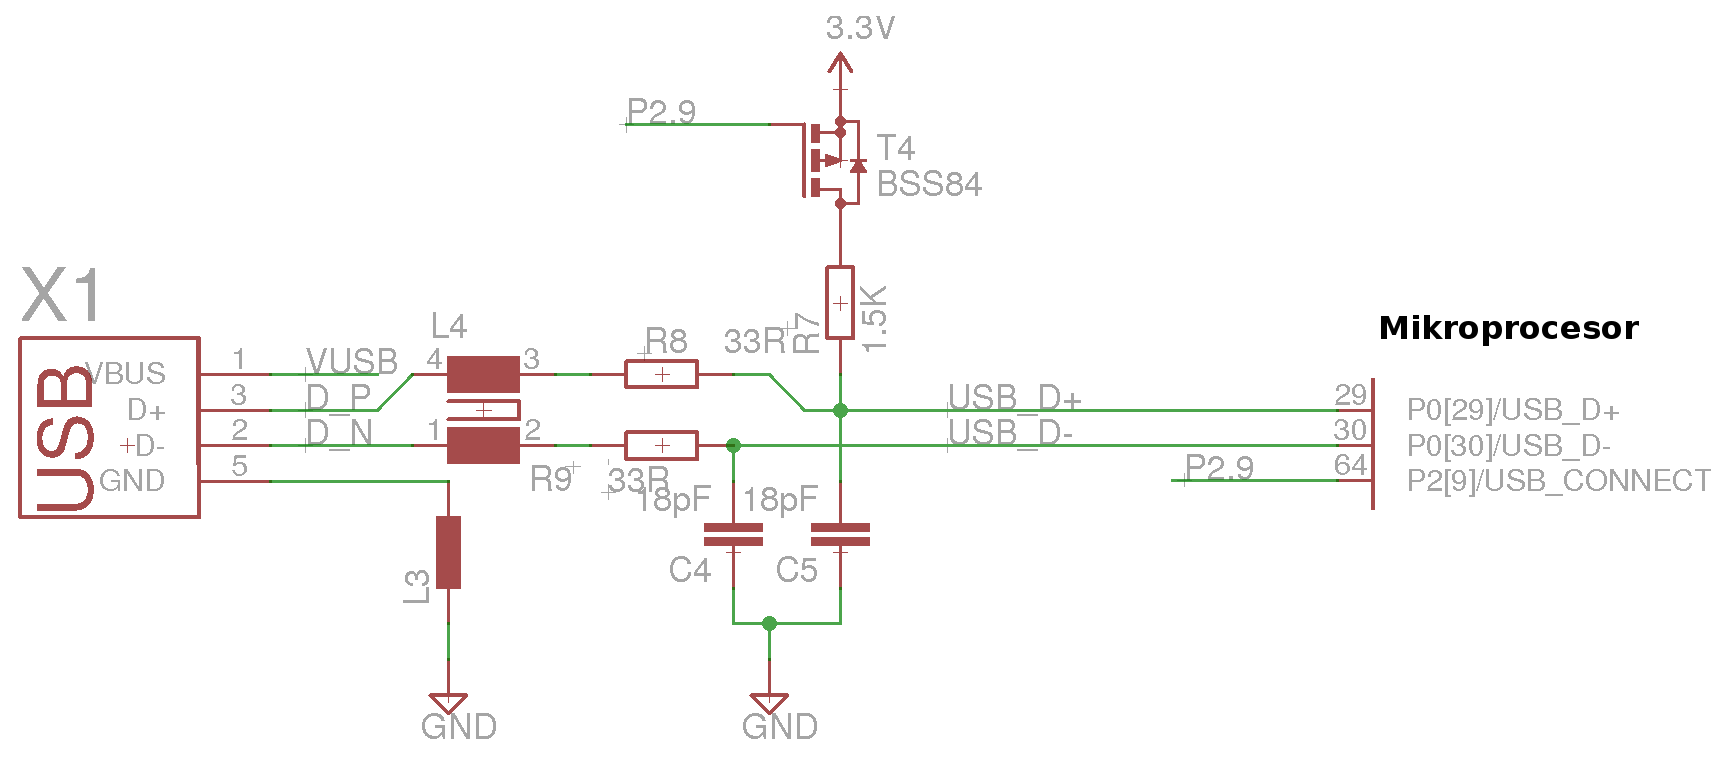
\includegraphics[width=0.8\linewidth]{obrazky/usbEMI.png}%
    \caption{Zapojení USB.}
\end{figure}

V této kapitole byly vyzdviženy jen nejdůležitější části obvodu, celé schéma zapojení je pak možé najít v příloze A

\section{Zapojení konektorů}

\begin{figure}[h!]

  \centering
    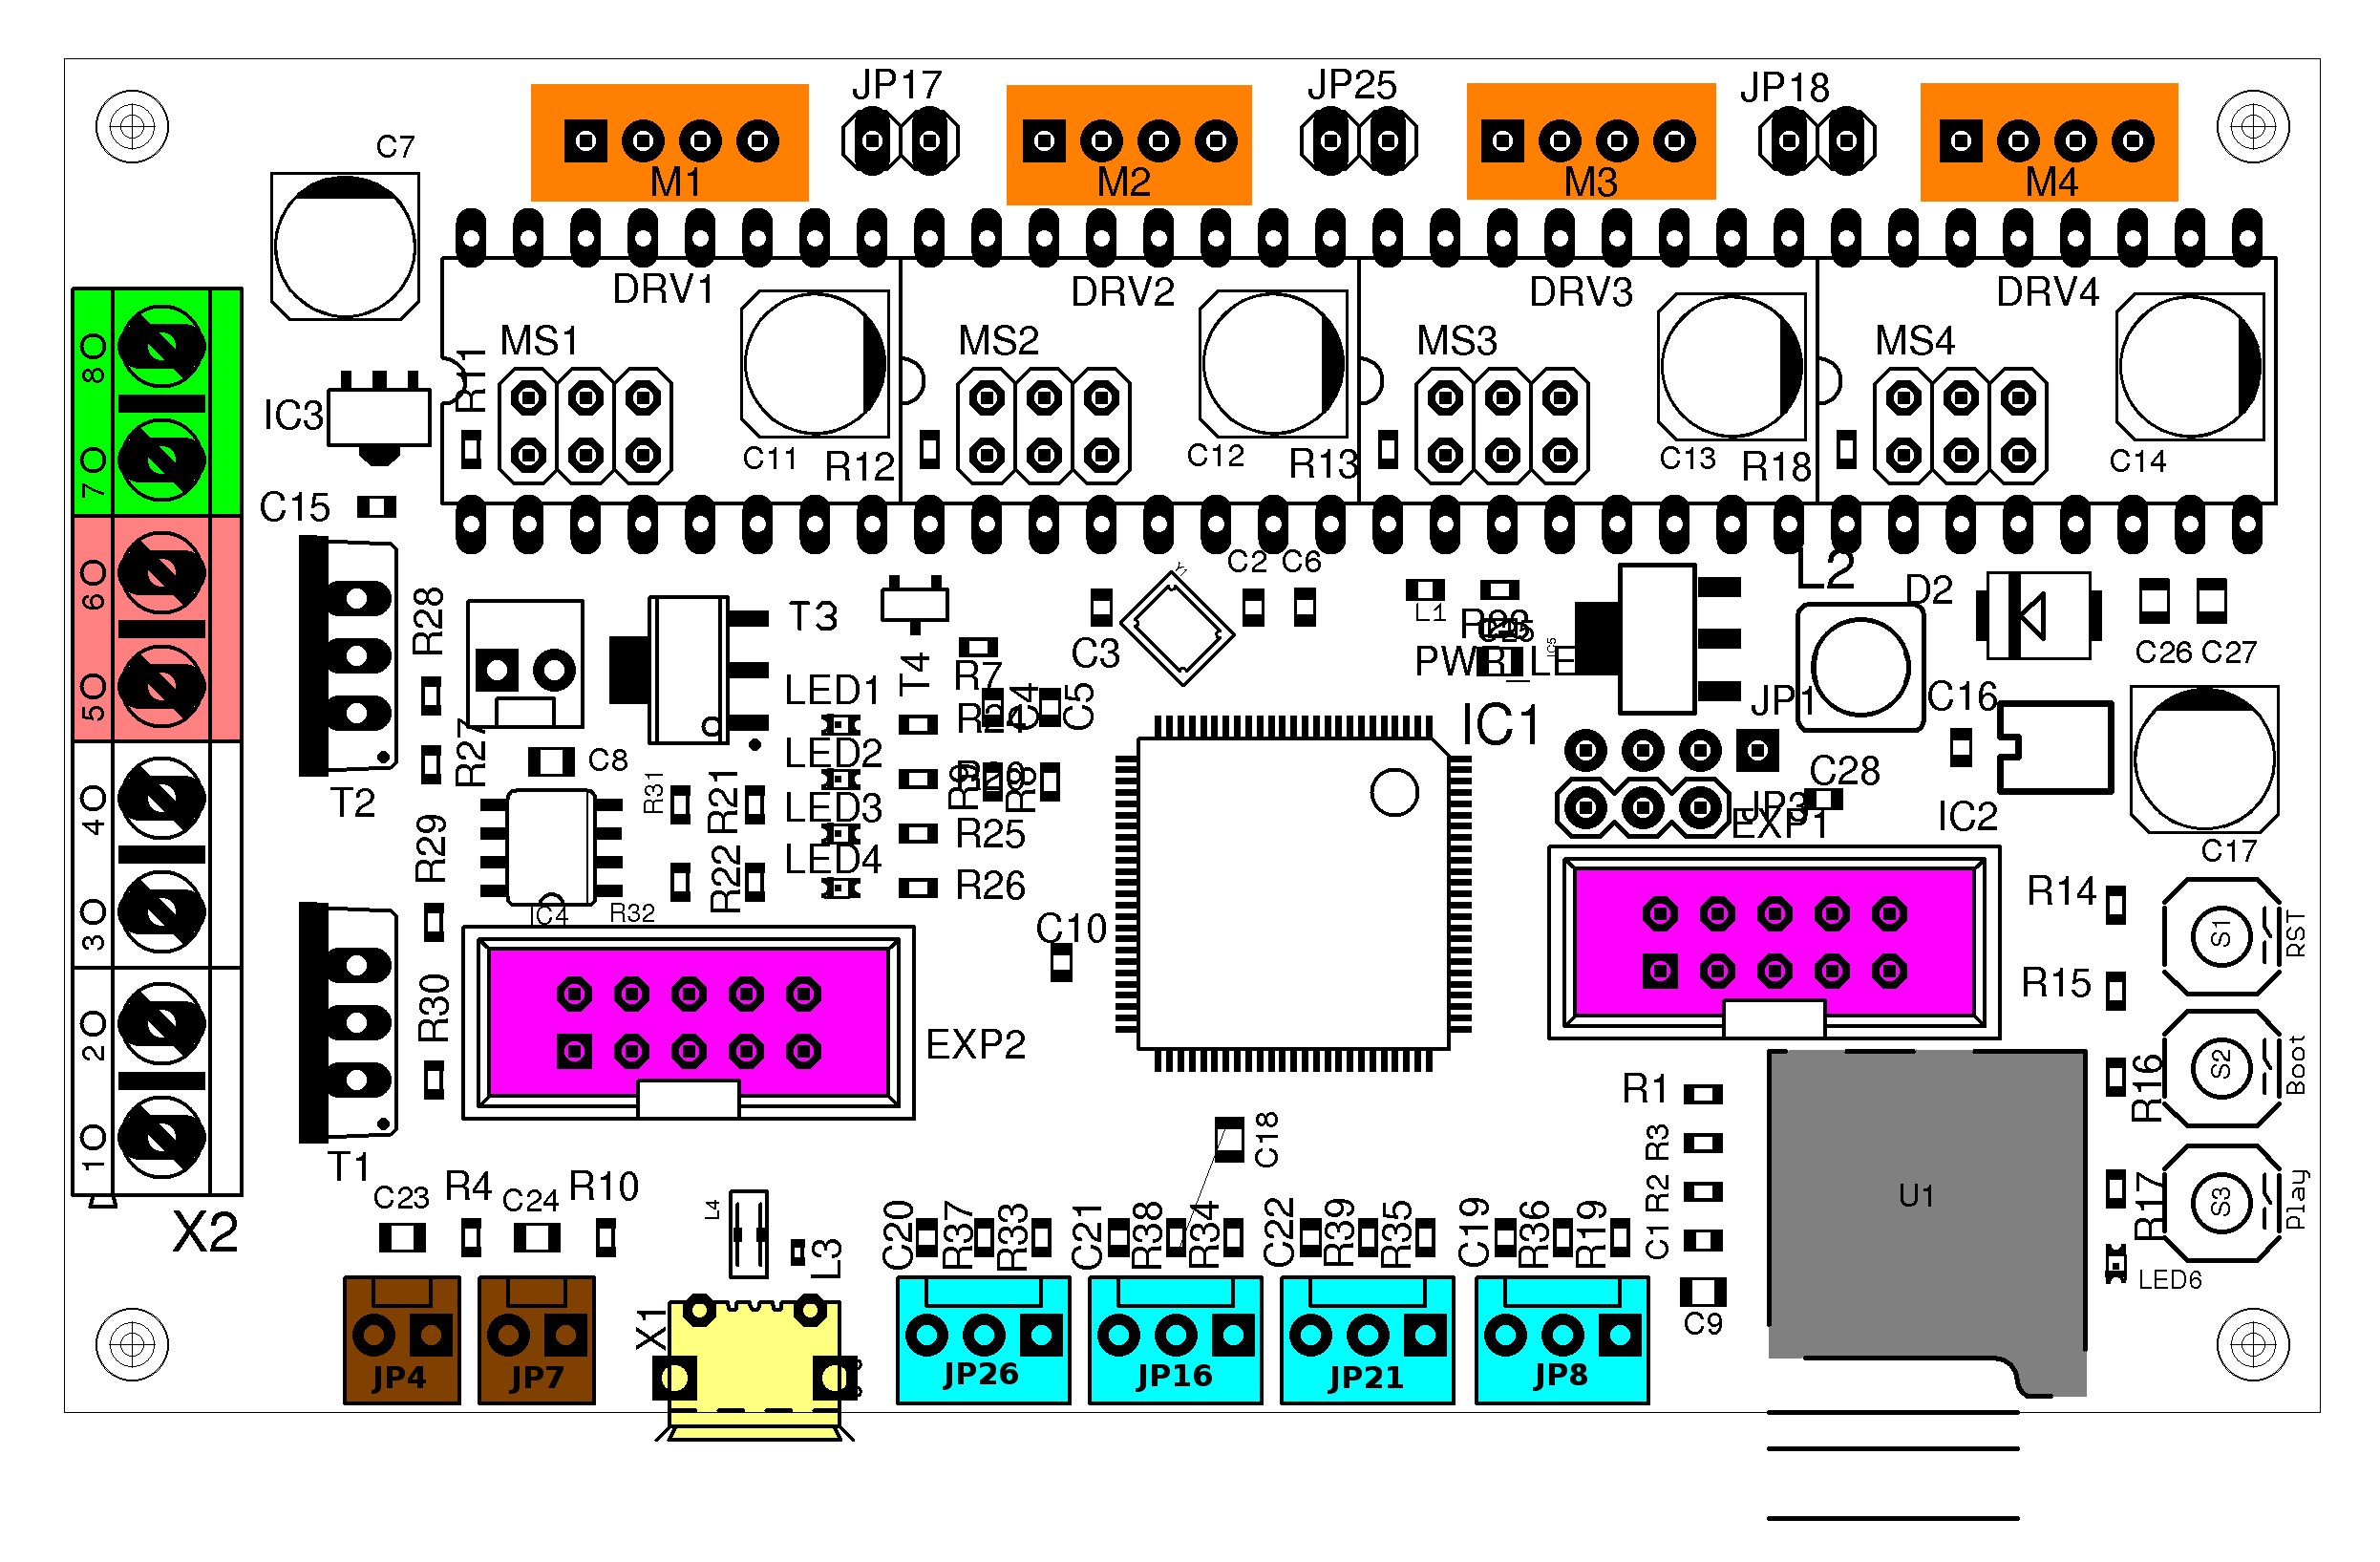
\includegraphics[width=0.8\linewidth]{obrazky/base3D_barva.png}%
    \caption{Zapojení konektorů.}
\end{figure}



\begin{table}[h!]
  \caption{Zapojení konektorů. }
  \begin{center}
  	\small
	  \begin{tabular}{|c|c|c|}
	    \hline
	    Barva			& Reference			& Význam  					\\
	    \hline\hline
		\cellcolor{blue!25}- 			& M1, M2, M3, M4		& Motory X, Y, Z a R				\\
		\hline
		-			& U1				& SD karta					\\
		\hline
		-			& X1				& USB konektor pro propojení s PC		\\
		\hline
		-			& X2-7, X2-8			& Napájení +24V					\\
		\hline
		-			& X2-5, X2-6			& Ventil pro řízení vakua			\\
		\hline
		-			& EXP1, EXP2			& Konektory pro připojení externího displaye	\\
		\hline
		-			& JP4, JP7			& ADC pro měření úrovně vakua 			\\
		\hline
	    \hline
	  \end{tabular}
  \end{center}
\end{table}

\begin{figure}[h!]

  \centering
    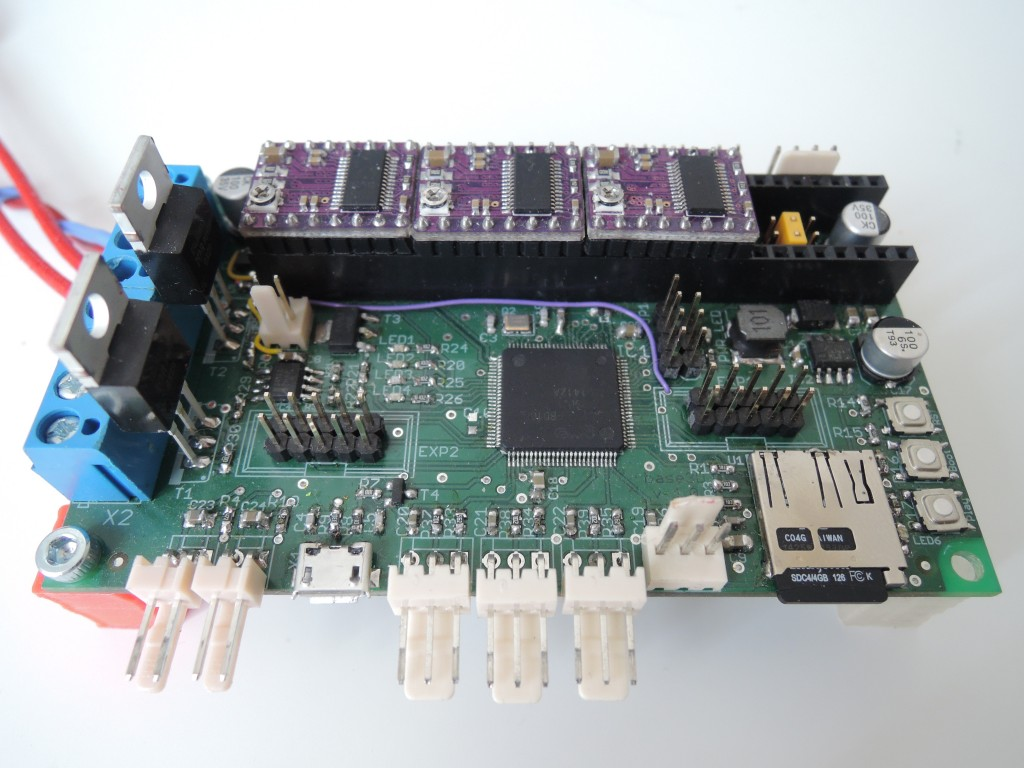
\includegraphics[width=0.8\linewidth]{obrazky/DSCN2185.JPG}%
    \caption{Osazená řídící elektronika ve verzi 1.0.}
\end{figure}




%% Vložení souboru 'text/sw' s popisem vysledků práce
\chapter{Řídící SW}

Řídící software pro osazovací automat byla nejtěžší část celého projektu. SW spojuje jednotlivé části popsané v předcházejících kapitolách do jednoho celku. 



Jeden z hlavních požadavků na řídící SW byla jeho platformová nezávislost. Tedy možnost spuštění aplikace jak na operačním systému Linux, tak i na Windows. Protože aplikace má grafické rozhraní, zúžil se výběr mnou známých programovacích jazyků na C/C++, Java, Delphi a Python. Byl vybrán  právě poslední zmiňovaný Python, jelikož má velice dobrou dokumentaci a nástroje pro tvorbu GUI jsou uživatelsky přívětivé.
Tato kombinace slibovala rychlý prototyping SW a naději na funkční SW. Pro tvorbu GUI padla volba na PyQt.

V aplikaci je kvůli centrování součástek a desek potřebné i vyhodnocování obrazu. Jako základ byla použita hojně používaná knihovna OpenCV. Ta nabízí set základních funkcí pro manipulaci s obrazem. Implementované funkce jako rozostření, hledání hran, kontur a kruhů zjednoduší úlohu rozpoznávání pozice a rotace součástek a hledání centrovacích bodů DPS.


Screenshoty z QTGUI a pár věcí ohledně PyQt







\section{Data pro osazovací automat}

Pro návrh elektronických systémů se používá software spadající do kategorie EDA – Electronic Design Automation. Je to soubor nástrojů pro tvorbu desek plošných spojů (a integrovaných obvodů). Mezi základní nástroje patří Schématické editory, simulátory obvodů, autoroutery, návrhové prostředí pro tvorbu DPS a CAM procesor. 
Příkladem EDA softwérů jsou: Altium Designer, KiCad, CadSoft Eagle.

Pro testování byl použit poslední zmiňovaný CadSoft Eagle, který je ve své základní varianě pro nekomerční účely dostupný zdarma. Uvžujme vytvořené schéma a DPS. Pro osazovací automat potřebujeme získat pozici, hodnotu, typ pouzdra a rotaci každé SMD součástky, dále potřebujeme získat pozici centrovacích značek. K tomu se částečně dají použít jendak vestavěné funkce, Eagle ale disponuje i možností použití tzv ULP (User Language Program. ) skriptů. ULP je programovací jazyk postavený na základech C a umožňuje přímé modifikování schématu, DPS a vytváření různých exportů.


Vestavěný export
Jednou z cest jak vyexportovat pozice součástek je \verb|File->Export->Partlist|


Výsledný export obsahuje všechny použité součástky a exportované pozice jsou v jednotkách mil. Pro osazovací automat je ale potřeba jen SMD součástek a centrovacích bodů. Tento export tedy není příliš vhodný, protože by potřeboval ještě následnou ruční úpravu spočívající minimálně v odmazání všech THD součástek


\begin{table}[h!]
  \caption{Ukázka exportu. }
  \begin{center}
  	\small
	  \begin{tabular}{|c|c|c|c|c|c|}
	    \hline
	    Part	& Value 	& Package 	& Library 	& Position (mil) 	& orientation	\\
	    \hline\hline

		C1 	& .1uF		& C0603		& resistor	& (2860 300)		& R180		\\
		\hline
		C2 	& 18pF		& C0603		& rcl		& (2075 1405)		& R90		\\
		\hline
	    \hline
	  \end{tabular}
  \end{center}
\end{table}

Součástí instalace Eagle je i několik již připravených ULP skriptů pro export, například Centroid\_ScreamingCircuits\_smd.ulp
Ten generuje oproti Partlistu strojově čitelnější formát a exportuje jen SMD součástky. Bohužel však chybí typ použitého pouzdra a hodnota součástky. 

\begin{verbatim}
  RefDes,Layer,LocationX,LocationY,Rotation
  C1,Top,2.860,0.300,180
  C2,Top,2.075,1.405,90
\end{verbatim}

Pro vytvoření exportu se všemi potřebnými hodnotami tak bylo potřeba napsat vlastní ULP skrip. 
Ten exportuje středy/origins součástek tak, jak byly vytvořené autorem součástky v knihovnách, dále i geomterické středy součástek. Geomterický střed funguje tak, že se iteruje nad všemi ploškami součástky a hledá se minimum a maximum v obou osách. Jejich rozdíl se vydělí dvěma a najde se skutečný střed součástky. Není to tak střed součástky základě geometrického tvaru pouzdra! Na to je třeba brát později zřetel. Důvod pro export těchto souřadnic je ten, že né všechny součástky v knihovnách se drží zažitého standardu na umisťování středícího bodu do středu pouzdra, případně do levého horního rohu.

Ukázka z ULP skriptu exportující informace o centrovacích bodech DPS

\begin{verbatim}
  printf("Part name;Package;Value;X origin;Y origin;\n");
  printf("%%fiducials\n");
  B.elements(E) if (E.populate) {

    if (E.package.name == "FIDUCIAL_1MM") 
         printf("%s;%s;%s;%.3f;%.3f;\n",
         E.name, E.package.name, E.value, u2mm(E.x), u2mm(E.y));  


  }
  printf("%%end_fiducials\n");
\end{verbatim}

Výsledný export je pak ve formátu 
\begin{verbatim}
  %data
  Part name;X center;Y center;X origin;Y origin;Rotation;Value;Package
  C1;72.644;7.620;72.644;7.620;180;.1uF;C0603
  C2;52.705;35.687;52.705;35.687;90;18pF;C0603
  %data_end
  %fiducials
  Part name;Package;Value;X origin;Y origin;
  U$3;FIDUCIAL_1MM;FIDUCIAL;7.500;3.000;
  U$4;FIDUCIAL_1MM;FIDUCIAL;7.500;57.000;
  U$6;FIDUCIAL_1MM;FIDUCIAL;92.500;3.000;
  %fiducials_end
\end{verbatim}

skript také exportuje obrázek dané DPS, který se dá po načtení do řídícího SW použít pro simulaci osazování. Celý skript je přiložen v příloze B.



%% Vložení souboru 'text/vysledky' s popisem vysledků práce
\chapter{Měření}

\section{Přesnost}
\section{Reprodukovatelnost}
Reprodukovatelnost mechanismu je po přesnosti pozicování dalším z klíčovým parametrem. Přesnost a reprodukovatelnost jsou spolu úzce spojeny. Reprodukovatelnost je definována jako schopnost mechanismu vracet se zpet na dané místo znovu a znovu. 
Meření bylo založeno na metodě popsané v \cite{vaske}. Měření probíhá tak, že ve středu souřadnicového systému je stanovena reference. Z této pozice je prováděn pohyb do krajních pozic mechanismu a zpět. Právě kvůli chybě reprodukovatelnosti pohybů není pokaždé možné najet na přesně stejnou pozici. Proto je po každém pohybu zpět stanovena nová reference. Jednotlivé vásledky se tak neporovnávají vůči počáteční pozici, ale porovnávají se mezi sebou dvě poslední pozice reference.  

Na obrázku \cite{fig:repeatability} je vidět souřadnicová sít s naznačenými pozicemi jednotlivých pohybů. Celý test je naprogramovaný přímo do řídícího SW a je ho možné kdykoliv spustit.

\begin{figure}[h!]
  \centering
    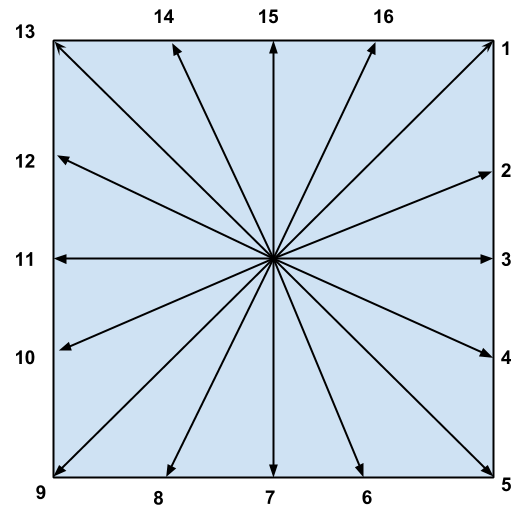
\includegraphics[width=0.9\linewidth]{obrazky/repeatability.png}%
    \caption{Repeatabilita TODO.}
    \label{fig:repeatability}
\end{figure}




%% Vložení souboru 'text/zaver' se závěrem
\chapter{Závěr}

Limitace velikost soucastek, nedostatek vakua. 



SW:
Mnou stanovený požadavek na multiplatformí SW byl splněn, ale bohužel nedošlo na jeho verifikaci v praxi. Všechny testy byly prováděny pouze na operačním systému Fedora 21 (Linux).  Možná inkompatibilita hrozila v různém přístupu systémů k hardware, konkrétně k sériovému portu a dále v kompatibilitě grafického rozhraní. Pro eliminaci problémů s HW byla použita knihovna PySerial, která je dostupná ve verzích pro Windows, Linux i MacOS/X. Stejně tak použitý framework na grafické rozhraní PyQt je dostupný pro již zmíněně operační systémi.
Při spoušění programu na jiných platformách než Linux se tak nepředpokládají žádné problémy.
\\

HW:
Při návrhu a následném testování elektroniky jsem získal velice cenné zkušenosti z oblasti elektromagnetické kompatibility. První prototyp navržené elektroniky byl náchylný na elektromagnetickou susceptibilitu a z toho důvodu docházelo k výpadkům komunkace přes USB rozhraní. Po nastudování nesčetných zdrojů se povedlo v druhé revizi problém eliminovat. A to za pomocí filtrů na signálových cestách a striktním dodržení návrhových pravidel daných výrobcem mikrokontroléru.
\\

Využití:
Jak bylo naznačeno v kapitole XXX, osazovací automat může být po úpravě řídícího SW využit i pro automatickou optickou inspekci (AOI) osazených a zapájených DPS. Spojil by tak dva kroky výrobního procesu DPS do jednoho přístroje.
Realizovaná konstrukce je poměrně univerzální a mohla by najít využítí také jako manipulační robot.


%% Vložení souboru 'text/literatura' se seznamem literatury
\begin{literatura}{99}
	
\bibitem{boldis}
    BOLDIŠ, P.
    \emph{Bibliografické citace dokumentů podle ČSN ISO 690 a ČSN ISO 690-2}\/ [online].
    2001, poslední aktualizace 11.\,11.\,2004 [cit.\,17.\,2.\,2005].
    Dostupné z~URL:
    \(<\)\url{http://www.boldis.cz/citace/citace.html}\(>\).
	

\bibitem{intel}
    INTEL CORPORATION.
    \emph{Power Delivery Design Issues for Hi-Speed USB on Motherboards}\/ [online].
    2002 [cit.\,10.\,3.\,2015].
    Dostupné z~URL:
    \(<\)\url{http://www.usb.org/}\(>\).

\bibitem{vaske}
    Vaške, F.
    \emph{Design and implementation of testing device for gonio mechanisms}\/ .
    2012.



\end{literatura}


%% Vložení souboru 'text/zkratky' se seznam použitých symbolů, veličin a zkratek
\begin{seznamzkratek}{KolikMista}



	\novazkratka{zkPCB}		% název
		{PCB}								% zkratka
		{Deska plošných spojů}
											% rozvinutí zkratky

	\novazkratka{zkAOI}						% název
		{AOI} % symbol
		{Automatická Optická Inspekce}					% popis

	\novazkratka{zkPnP}						% název
		{PnP} % symbol
		{Pick and Place}					% popis

	\novazkratka{zkUSB}						% název
		{USB} % symbol
		{Universal Serial Bus}					% popis
		
\end{seznamzkratek}


%% Začátek příloh
\prilohy

%% Vysázení seznamu příloh
\seznampriloh

%% Vložení souboru 'text/prilohy' s přílohami
\chapter{Některé příkazy balíčku \texttt{thesis}}\label{priloha:A}

\section{Příkazy pro sazbu veličin a jednotek}

\begin{table}[!h]
  \caption{Přehled příkazů pro matematické prostředí }
  \begin{center}
  	\small
	  \begin{tabular}{|c|c|c|c|}
	    \hline
	    Příkaz    						& Příklad 					& Zdroj příkladu  							& Význam  \\
	    \hline\hline
	    \verb|\textind{...}|	& $\beta_\textind{max}$ 	& \verb|$\beta_\textind{max}$|	& textový index \\
	    \hline
	    \verb|\konst{...}| 		& $\konst{U}_\textind{in}$ 				& \verb|$\konst{U}_\textind{in}$|		& konstantní veličina \\
	    \hline
	    \verb|\prom{...}| 		& $\prom{u}_\textind{in}$ & \verb|$\prom{u}_\textind{in}$| & proměnná veličina \\
	    \hline
	    \verb|\komplex{...}| 	& $\komplex{u}_\textind{in}$ & \verb|$\komplex{u}_\textind{in}$| & komplexní veličina \\
	    \hline
	    \verb|\vekt{...}| 		& $\vekt{y}$ 						& \verb|$\vekt{y}$| & vektor \\
	    \hline
	    \verb|\matice{...}| 	& $\matice{Z}$ 						& \verb|$\matice{Z}$| & matice \\
	    \hline
	    \verb|\jedn{...}| 		& $\jedn{kV}$ 						& \verb|$\jedn{kV}$|\quad či\ \, \verb|\jedn{kV}| & jednotka \\
	    \hline
	  \end{tabular}
  \end{center}
\end{table}



%\newpage
\section{Příkazy pro sazbu symbolů}

\begin{itemize}
  \item
    \verb|\E|, \verb|\eul| -- sazba Eulerova čísla: $\eul$,
  \item
    \verb|\J|, \verb|\jmag|, \verb|\I|, \verb|\imag| -- sazba imaginární jednotky: $\jmag$, $\imag$,
  \item
    \verb|\dif| -- sazba diferenciálu: $\dif$,
  \item
    \verb|\sinc| -- sazba funkce: $\sinc$.
  \item
    \verb|\mikro| -- sazba symbolu mikro stojatým písmem\footnote{znak pochází z~balíčku \texttt{textcomp}}: $\mikro$.

\end{itemize}
%
Všechny symboly jsou určeny pro matematický mód, vyjma \verb|\mikro|, jenž je použitelný rovněž v~textovém módu.






\chapter{Osazené DPS}\label{priloha:B}


\section{Testovací DPS C}
\begin{figure}[H]
  \centering
    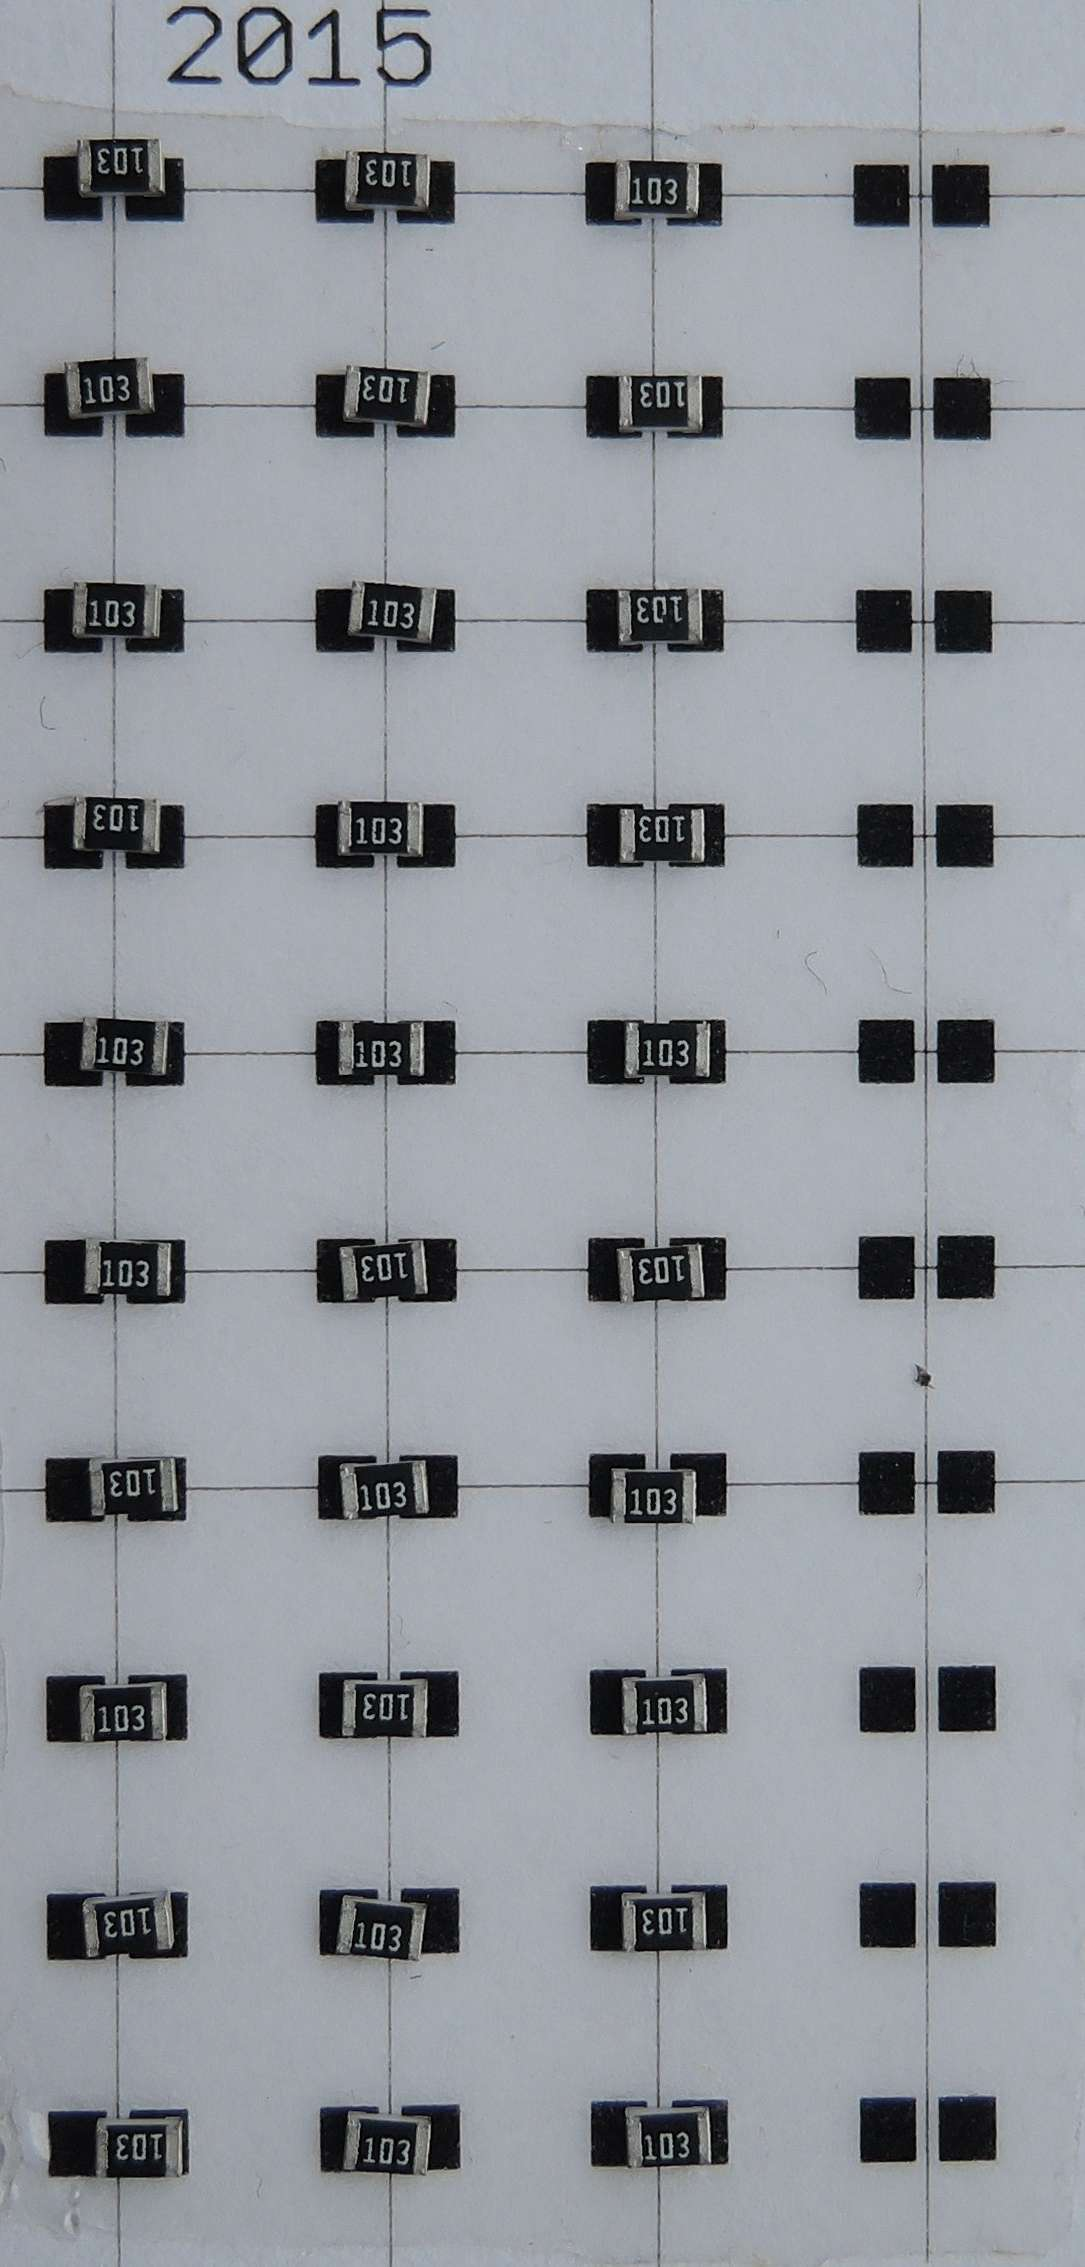
\includegraphics[height=0.35\paperheight ]{obrazky/C2.jpg}%
    \caption{Testovací DPS C.}
    \label{img:DeskaC}
\end{figure}


\begin{table}[H]
  \caption{Naměřené chyby osazení pro testovací DPS C.}
  \begin{center}
  	\small
	  \begin{tabular}{|c|c|c|c|c|c|c|c|c|c|c|}
	    \hline
			& \textbf{R41}	& \textbf{R42}	& \textbf{R43}	& \textbf{R44}	& \textbf{R45}	& \textbf{R46}	& \textbf{R47}	& \textbf{R48}	& \textbf{R49}	& \textbf{R50}  \\
	    \hline
	    \textbf{x}	& 0,455&	0,364&	0,242&	0,364&	0,121&	0,091&	0,091&	0,030&	0,182&	0,06  \\
	    \hline
	    \textbf{y}	&0,212&	0,091&	0,182&	0,061&	0,364&	0,455&	0,545&	0,273&	0,212&	0,515 \\
	    \hline
			& \textbf{R51}	& \textbf{R52}	& \textbf{R53}	& \textbf{R54}	& \textbf{R55}	& \textbf{R56}	& \textbf{R57}	& \textbf{R58}	& \textbf{R59}	& \textbf{R60}  \\
	    \hline
	    \textbf{x}	&0,182&	0,212&	0,212&	0,212&	0,182&	0,000&	-0,030&	0,030&	-0,152&	0,061  \\
	    \hline
	    \textbf{y}	&0,091&	0,030&	0,303&	-0,061&	-0,030&	0,030&	-0,061&	-0,061&	-0,182&	0,030 \\
	    \hline
	    		& \textbf{R61}	& \textbf{R62}	& \textbf{R63}	& \textbf{R64}	& \textbf{R65}	& \textbf{R66}	& \textbf{R67}	& \textbf{R68}	& \textbf{R69}	& \textbf{R70}  \\
	    \hline
	    \textbf{x}	& -0,030&	0,000&	0,061&	0,000&	0,000&	-0,061&	-0,333&	-0,030&	0,030&	-0,061 \\
	    \hline
	    \textbf{y}	& 0,000&	0,030&	-0,030&	0,000&	-0,152&	0,000&	-0,091&	0,061&	0,182&	0,152 \\
	    \hline
	  \end{tabular}
  \end{center}
\end{table}




\section{Testovací DPS D}
\begin{figure}[H]
  \centering
    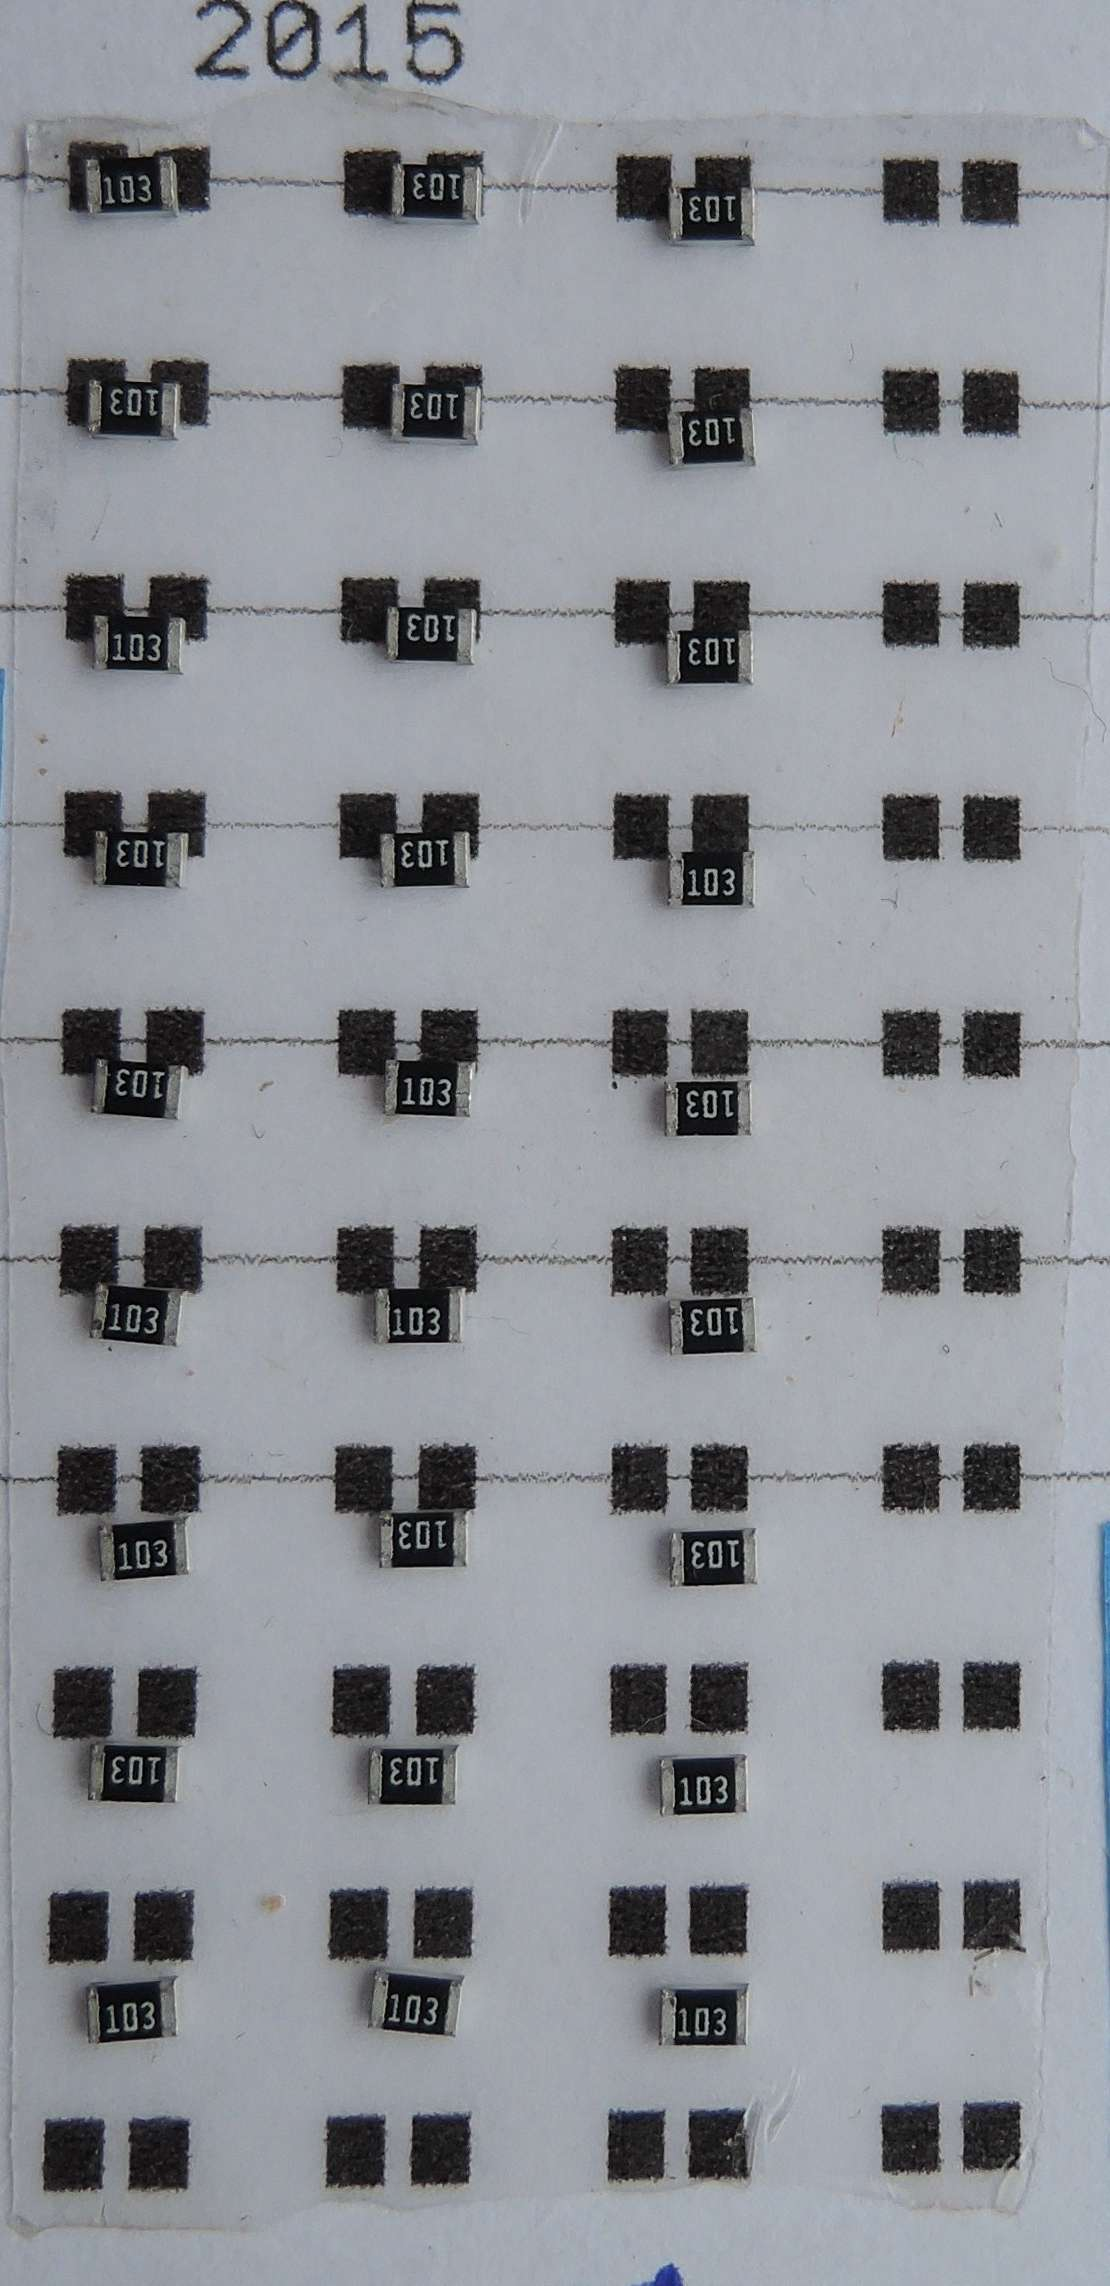
\includegraphics[height=0.35\paperheight ]{obrazky/D2.jpg}%
    \caption{Testovací DPS D.}
    \label{img:DeskaD}
\end{figure}


\begin{table}[H]
  \caption{Naměřené chyby osazení pro testovací DPS D.}
  \begin{center}
  	\small
	  \begin{tabular}{|c|c|c|c|c|c|c|c|c|c|c|}
	    \hline
			& \textbf{R41}	& \textbf{R42}	& \textbf{R43}	& \textbf{R44}	& \textbf{R45}	& \textbf{R46}	& \textbf{R47}	& \textbf{R48}	& \textbf{R49}	& \textbf{R50}  \\
	    \hline
	    \textbf{x}	& -0,515&	-0,485&	-1,121&	-0,818&	-1,121&	-1,424&	-1,758&	-1,576&	-1,970&	na \\
	    \hline
	    \textbf{y}	&-0,182&	-0,182&	0,212&	0,030&	0,061&	0,242&	0,576&	0,182&	0,455&	na \\
	    \hline
			& \textbf{R51}	& \textbf{R52}	& \textbf{R53}	& \textbf{R54}	& \textbf{R55}	& \textbf{R56}	& \textbf{R57}	& \textbf{R58}	& \textbf{R59}	& \textbf{R60}  \\
	    \hline
	    \textbf{x}	& -0,424&	-0,455&	-0,545&	-0,848&	-1,273&	-1,485&	-1,364&	-1,697&	-1,939&	na  \\
	    \hline
	    \textbf{y}	& 0,545&	0,545&	0,485&	0,333&	0,515&	0,242&	0,364&	0,182&	0,394&	na \\
	    \hline
	    		& \textbf{R61}	& \textbf{R62}	& \textbf{R63}	& \textbf{R64}	& \textbf{R65}	& \textbf{R66}	& \textbf{R67}	& \textbf{R68}	& \textbf{R69}	& \textbf{R70}  \\
	    \hline
	    \textbf{x}	& -0,727&	-1,030&	-1,152&	-1,394&	-1,667&	-1,606&	-1,970&	-2,091&	-2,182&	na \\
	    \hline
	    \textbf{y}	& 0,636&	0,667&	0,667&	0,788&	0,636&	0,758&	0,758&	0,636&	0,667&	na \\
	    \hline

	  \end{tabular}

  \end{center}

\end{table}







\section{Testovací DPS E}
\begin{figure}[H]
  \centering
    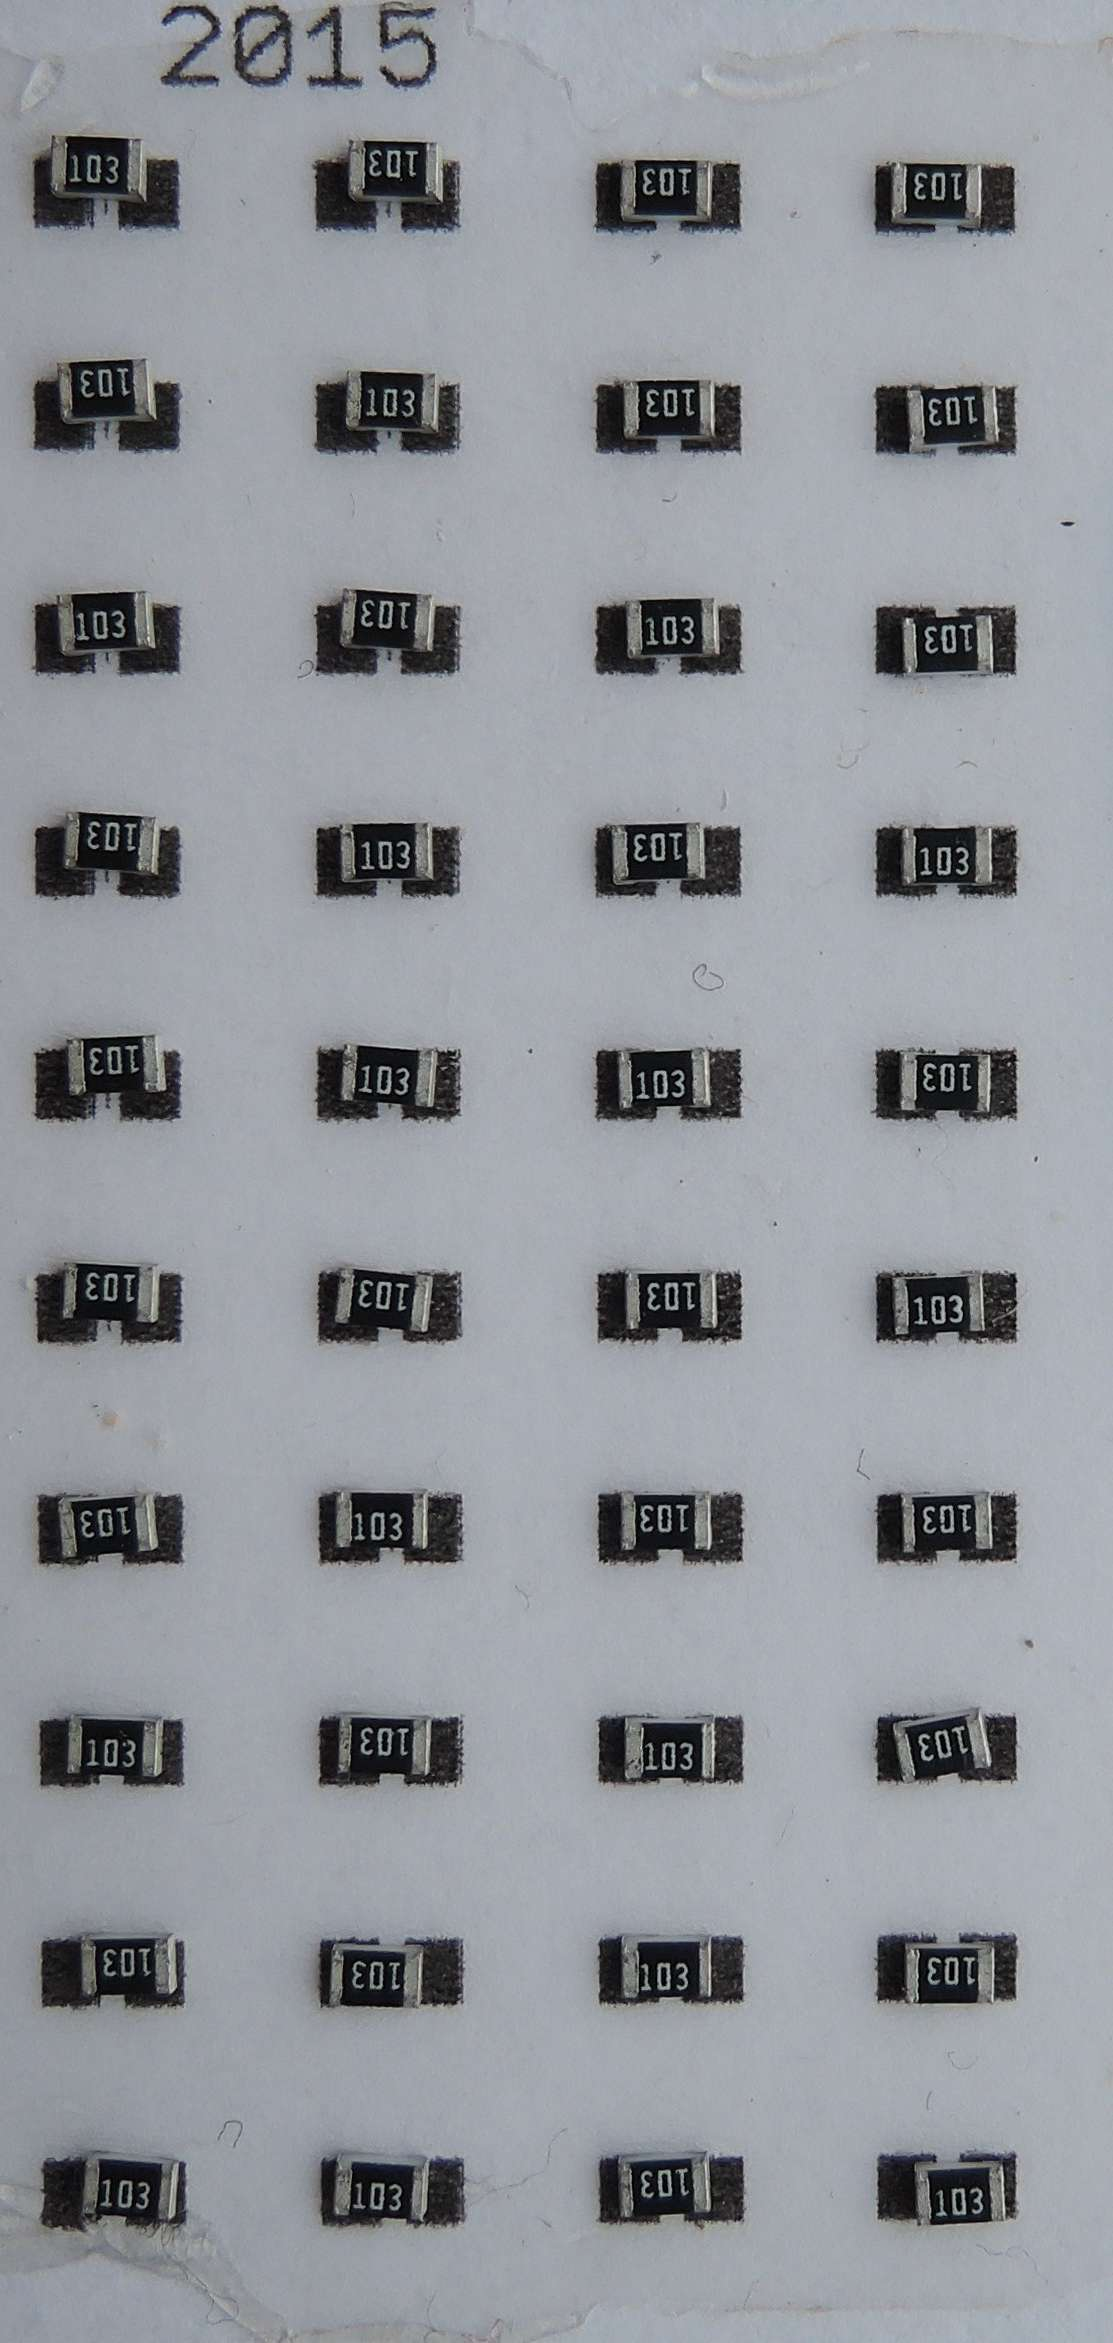
\includegraphics[height=0.35\paperheight ]{obrazky/E2.jpg}%
    \caption{Testovací DPS E.}
    \label{img:DeskaE}
\end{figure}



\begin{table}[H]
  \caption{Naměřené chyby osazení pro testovací DPS E.}
  \begin{center}
  	\small
	  \begin{tabular}{|c|c|c|c|c|c|c|c|c|c|c|}
	    \hline
			& \textbf{R41}	& \textbf{R42}	& \textbf{R43}	& \textbf{R44}	& \textbf{R45}	& \textbf{R46}	& \textbf{R47}	& \textbf{R48}	& \textbf{R49}	& \textbf{R50}  \\
	    \hline
	    \textbf{x}	& 0,515	& 0,515	& 0,424	& 0,394	& 0,485	& 0,515	& 0,303	& 0,273	& 0,333	& 0,333 \\
	    \hline
	    \textbf{y}	&-0,030	& 0,242	& 0,091	& 0,212	& 0,364	& 0,303	& -0,030 & 0,273 & 0,515& 0,576 \\
	    \hline
			& \textbf{R51}	& \textbf{R52}	& \textbf{R53}	& \textbf{R54}	& \textbf{R55}	& \textbf{R56}	& \textbf{R57}	& \textbf{R58}	& \textbf{R59}	& \textbf{R60}  \\
	    \hline
	    \textbf{x}	& 0,545	& 0,333	& 0,515	& 0,182	& 0,242	& 0,333	& 0,333	& 0,333	& 0,091	& 0,242  \\
	    \hline
	    \textbf{y}	& 0,333	& 0,273	& 0,152	& 0,061	& -0,030& -0,182& -0,242& -0,152& -0,364& -0,242 \\
	    \hline
	    		& \textbf{R61}	& \textbf{R62}	& \textbf{R63}	& \textbf{R64}	& \textbf{R65}	& \textbf{R66}	& \textbf{R67}	& \textbf{R68}	& \textbf{R69}	& \textbf{R70}  \\
	    \hline
	    \textbf{x}	& 0,000	& 0,152	& 0,212	& 0,333	& 0,121	& 0,273	& 0,242	& 0,030	& 0,061	& -0,333 \\
	    \hline
	    \textbf{y}	& 0,000	& -0,030& 0,121	& -0,273& 0,000	& -0,061& 0,030	& 0,000	& 0,000	& 0,212 \\
	    \hline

	  \end{tabular}

  \end{center}

\end{table}


\chapter{Obsah přiloženého CD}\label{priloha:C}

Nezapomeňte uvést, co čtenář najde na přiloženém médiu.
Je vhodné okomentovat obsah každého adresáře, specifikovat, který soubor obsahuje důležitá nastavení, který soubor je určen ke spuštění atd.
Také je dobře napsat, v~jaké verzi software byl kód testován (např.\ Matlab 2010b).


%% Konec dokumentu
\end{document}
